\documentclass[1p]{elsarticle_modified}
%\bibliographystyle{elsarticle-num}

%\usepackage[colorlinks]{hyperref}
%\usepackage{abbrmath_seonhwa} %\Abb, \Ascr, \Acal ,\Abf, \Afrak
\usepackage{amsfonts}
\usepackage{amssymb}
\usepackage{amsmath}
\usepackage{amsthm}
\usepackage{scalefnt}
\usepackage{amsbsy}
\usepackage{kotex}
\usepackage{caption}
\usepackage{subfig}
\usepackage{color}
\usepackage{graphicx}
\usepackage{xcolor} %% white, black, red, green, blue, cyan, magenta, yellow
\usepackage{float}
\usepackage{setspace}
\usepackage{hyperref}

\usepackage{tikz}
\usetikzlibrary{arrows}

\usepackage{multirow}
\usepackage{array} % fixed length table
\usepackage{hhline}

%%%%%%%%%%%%%%%%%%%%%
\makeatletter
\renewcommand*\env@matrix[1][\arraystretch]{%
	\edef\arraystretch{#1}%
	\hskip -\arraycolsep
	\let\@ifnextchar\new@ifnextchar
	\array{*\c@MaxMatrixCols c}}
\makeatother %https://tex.stackexchange.com/questions/14071/how-can-i-increase-the-line-spacing-in-a-matrix
%%%%%%%%%%%%%%%

\usepackage[normalem]{ulem}

\newcommand{\msout}[1]{\ifmmode\text{\sout{\ensuremath{#1}}}\else\sout{#1}\fi}
%SOURCE: \msout is \stkout macro in https://tex.stackexchange.com/questions/20609/strikeout-in-math-mode

\newcommand{\cancel}[1]{
	\ifmmode
	{\color{red}\msout{#1}}
	\else
	{\color{red}\sout{#1}}
	\fi
}

\newcommand{\add}[1]{
	{\color{blue}\uwave{#1}}
}

\newcommand{\replace}[2]{
	\ifmmode
	{\color{red}\msout{#1}}{\color{blue}\uwave{#2}}
	\else
	{\color{red}\sout{#1}}{\color{blue}\uwave{#2}}
	\fi
}

\newcommand{\Sol}{\mathcal{S}} %segment
\newcommand{\D}{D} %diagram
\newcommand{\A}{\mathcal{A}} %arc


%%%%%%%%%%%%%%%%%%%%%%%%%%%%%5 test

\def\sl{\operatorname{\textup{SL}}(2,\Cbb)}
\def\psl{\operatorname{\textup{PSL}}(2,\Cbb)}
\def\quan{\mkern 1mu \triangleright \mkern 1mu}

\theoremstyle{definition}
\newtheorem{thm}{Theorem}[section]
\newtheorem{prop}[thm]{Proposition}
\newtheorem{lem}[thm]{Lemma}
\newtheorem{ques}[thm]{Question}
\newtheorem{cor}[thm]{Corollary}
\newtheorem{defn}[thm]{Definition}
\newtheorem{exam}[thm]{Example}
\newtheorem{rmk}[thm]{Remark}
\newtheorem{alg}[thm]{Algorithm}

\newcommand{\I}{\sqrt{-1}}
\begin{document}

%\begin{frontmatter}
%
%\title{Boundary parabolic representations of knots up to 8 crossings}
%
%%% Group authors per affiliation:
%\author{Yunhi Cho} 
%\address{Department of Mathematics, University of Seoul, Seoul, Korea}
%\ead{yhcho@uos.ac.kr}
%
%
%\author{Seonhwa Kim} %\fnref{s_kim}}
%\address{Center for Geometry and Physics, Institute for Basic Science, Pohang, 37673, Korea}
%\ead{ryeona17@ibs.re.kr}
%
%\author{Hyuk Kim}
%\address{Department of Mathematical Sciences, Seoul National University, Seoul 08826, Korea}
%\ead{hyukkim@snu.ac.kr}
%
%\author{Seokbeom Yoon}
%\address{Department of Mathematical Sciences, Seoul National University, Seoul, 08826,  Korea}
%\ead{sbyoon15@snu.ac.kr}
%
%\begin{abstract}
%We find all boundary parabolic representation of knots up to 8 crossings.
%
%\end{abstract}
%\begin{keyword}
%    \MSC[2010] 57M25 
%\end{keyword}
%
%\end{frontmatter}

%\linenumbers
%\tableofcontents
%
\newcommand\colored[1]{\textcolor{white}{\rule[-0.35ex]{0.8em}{1.4ex}}\kern-0.8em\color{red} #1}%
%\newcommand\colored[1]{\textcolor{white}{ #1}\kern-2.17ex	\textcolor{white}{ #1}\kern-1.81ex	\textcolor{white}{ #1}\kern-2.15ex\color{red}#1	}

{\Large $\underline{12a_{0347}~(K12a_{0347})}$}

\setlength{\tabcolsep}{10pt}
\renewcommand{\arraystretch}{1.6}
\vspace{1cm}\begin{tabular}{m{100pt}>{\centering\arraybackslash}m{274pt}}
\multirow{5}{120pt}{
	\centering
	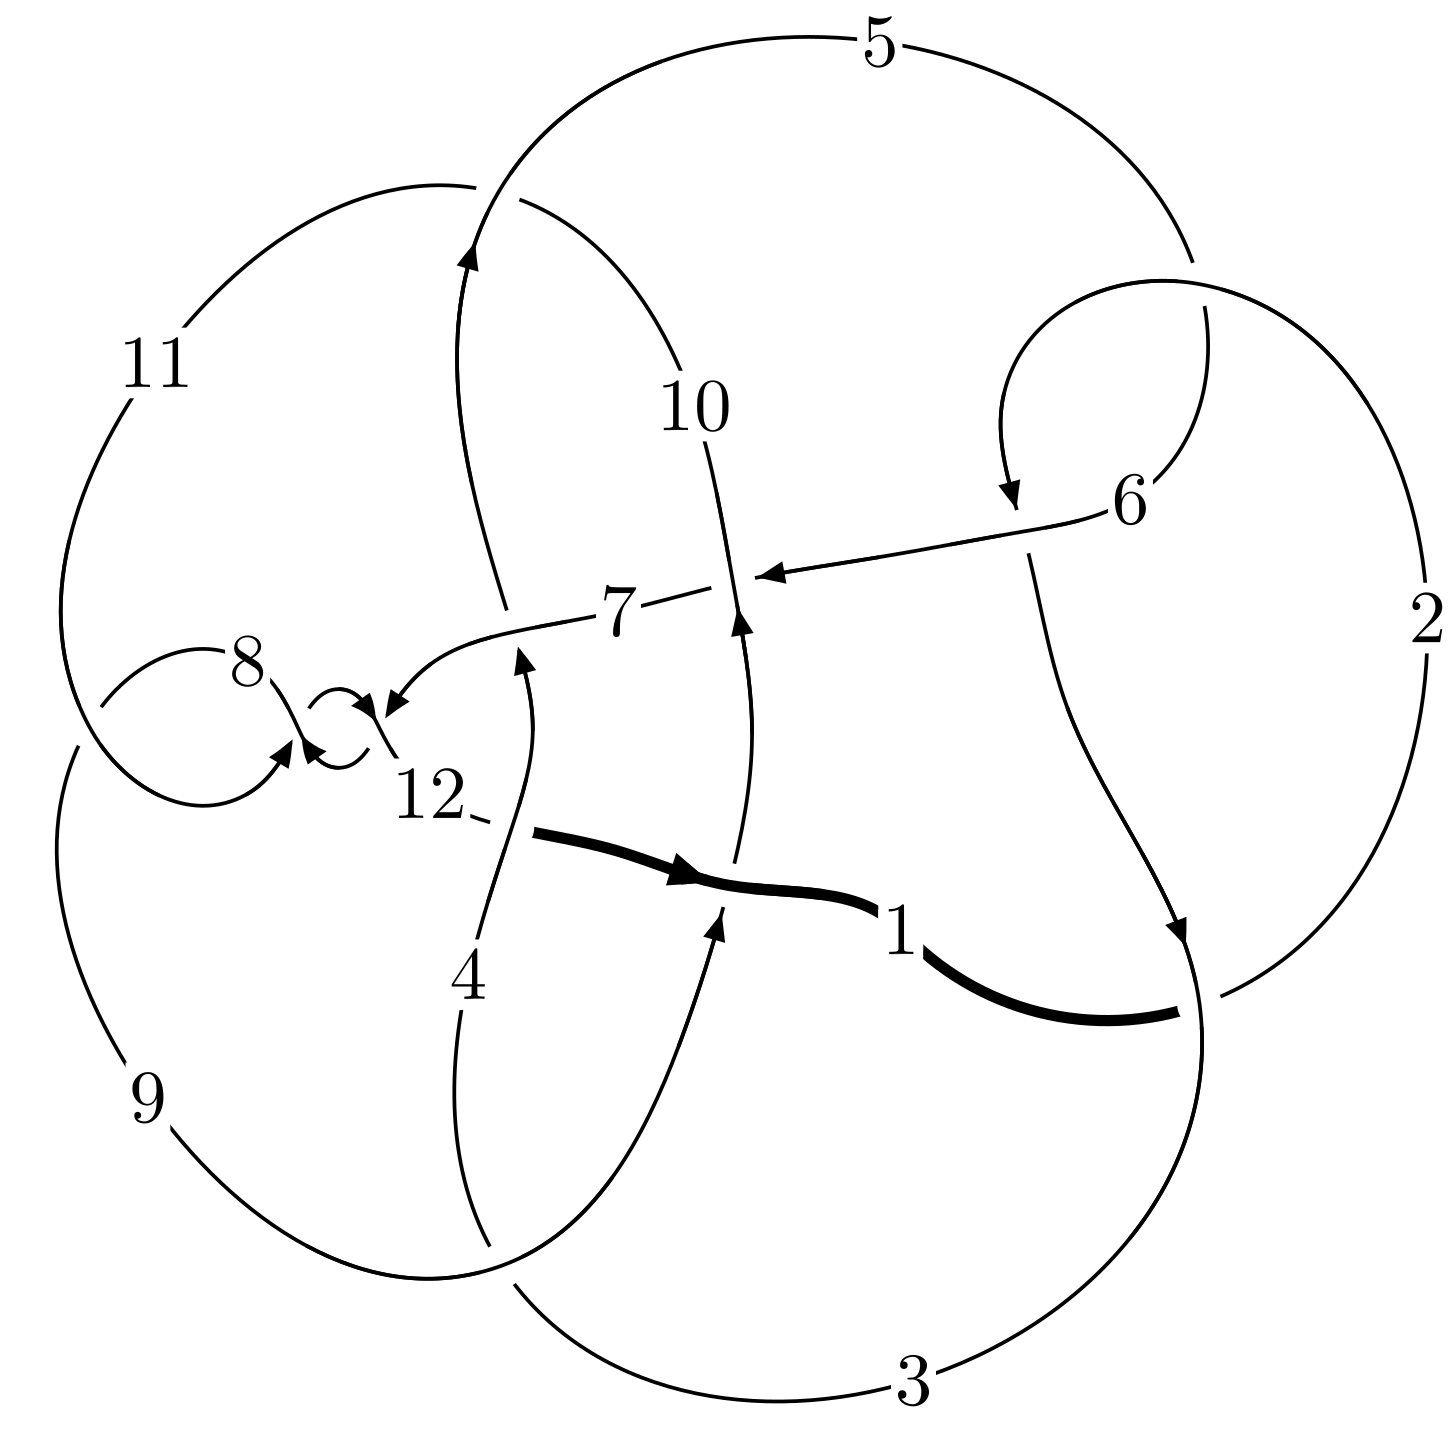
\includegraphics[width=112pt]{../../../GIT/diagram.site/Diagrams/png/1148_12a_0347.png}\\
\ \ \ A knot diagram\footnotemark}&
\allowdisplaybreaks
\textbf{Linearized knot diagam} \\
\cline{2-2}
 &
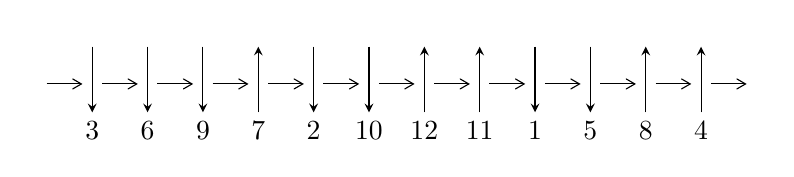
\begin{tikzpicture}[x=20pt, y=17pt]
	% nodes
	\node (C0) at (0, 0) {};
	\node (C1) at (1, 0) {};
	\node (C1U) at (1, +1) {};
	\node (C1D) at (1, -1) {3};

	\node (C2) at (2, 0) {};
	\node (C2U) at (2, +1) {};
	\node (C2D) at (2, -1) {6};

	\node (C3) at (3, 0) {};
	\node (C3U) at (3, +1) {};
	\node (C3D) at (3, -1) {9};

	\node (C4) at (4, 0) {};
	\node (C4U) at (4, +1) {};
	\node (C4D) at (4, -1) {7};

	\node (C5) at (5, 0) {};
	\node (C5U) at (5, +1) {};
	\node (C5D) at (5, -1) {2};

	\node (C6) at (6, 0) {};
	\node (C6U) at (6, +1) {};
	\node (C6D) at (6, -1) {10};

	\node (C7) at (7, 0) {};
	\node (C7U) at (7, +1) {};
	\node (C7D) at (7, -1) {12};

	\node (C8) at (8, 0) {};
	\node (C8U) at (8, +1) {};
	\node (C8D) at (8, -1) {11};

	\node (C9) at (9, 0) {};
	\node (C9U) at (9, +1) {};
	\node (C9D) at (9, -1) {1};

	\node (C10) at (10, 0) {};
	\node (C10U) at (10, +1) {};
	\node (C10D) at (10, -1) {5};

	\node (C11) at (11, 0) {};
	\node (C11U) at (11, +1) {};
	\node (C11D) at (11, -1) {8};

	\node (C12) at (12, 0) {};
	\node (C12U) at (12, +1) {};
	\node (C12D) at (12, -1) {4};
	\node (C13) at (13, 0) {};

	% arrows
	\draw[->,>={angle 60}]
	(C0) edge (C1) (C1) edge (C2) (C2) edge (C3) (C3) edge (C4) (C4) edge (C5) (C5) edge (C6) (C6) edge (C7) (C7) edge (C8) (C8) edge (C9) (C9) edge (C10) (C10) edge (C11) (C11) edge (C12) (C12) edge (C13) ;	\draw[->,>=stealth]
	(C1U) edge (C1D) (C2U) edge (C2D) (C3U) edge (C3D) (C4D) edge (C4U) (C5U) edge (C5D) (C6U) edge (C6D) (C7D) edge (C7U) (C8D) edge (C8U) (C9U) edge (C9D) (C10U) edge (C10D) (C11D) edge (C11U) (C12D) edge (C12U) ;
	\end{tikzpicture} \\
\hhline{~~} \\& 
\textbf{Solving Sequence} \\ \cline{2-2} 
 &
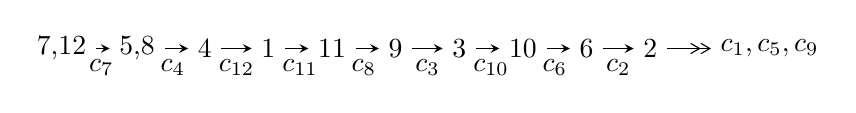
\begin{tikzpicture}[x=23pt, y=7pt]
	% node
	\node (A0) at (-1/8, 0) {7,12};
	\node (A1) at (17/16, 0) {5,8};
	\node (A2) at (17/8, 0) {4};
	\node (A3) at (25/8, 0) {1};
	\node (A4) at (33/8, 0) {11};
	\node (A5) at (41/8, 0) {9};
	\node (A6) at (49/8, 0) {3};
	\node (A7) at (57/8, 0) {10};
	\node (A8) at (65/8, 0) {6};
	\node (A9) at (73/8, 0) {2};
	\node (C1) at (1/2, -1) {$c_{7}$};
	\node (C2) at (13/8, -1) {$c_{4}$};
	\node (C3) at (21/8, -1) {$c_{12}$};
	\node (C4) at (29/8, -1) {$c_{11}$};
	\node (C5) at (37/8, -1) {$c_{8}$};
	\node (C6) at (45/8, -1) {$c_{3}$};
	\node (C7) at (53/8, -1) {$c_{10}$};
	\node (C8) at (61/8, -1) {$c_{6}$};
	\node (C9) at (69/8, -1) {$c_{2}$};
	\node (A10) at (11, 0) {$c_{1},c_{5},c_{9}$};

	% edge
	\draw[->,>=stealth]	
	(A0) edge (A1) (A1) edge (A2) (A2) edge (A3) (A3) edge (A4) (A4) edge (A5) (A5) edge (A6) (A6) edge (A7) (A7) edge (A8) (A8) edge (A9) ;
	\draw[->>,>={angle 60}]	
	(A9) edge (A10);
\end{tikzpicture} \\ 

\end{tabular} \\

\footnotetext{
The image of knot diagram is generated by the software ``\textbf{Draw programme}" developed by Andrew Bartholomew(\url{http://www.layer8.co.uk/maths/draw/index.htm\#Running-draw}), where we modified some parts for our purpose(\url{https://github.com/CATsTAILs/LinksPainter}).
}\phantom \\ \newline 
\centering \textbf{Ideals for irreducible components\footnotemark of $X_{\text{par}}$} 
 
\begin{align*}
I^u_{1}&=\langle 
-6.99189\times10^{50} u^{63}+7.06651\times10^{51} u^{62}+\cdots+5.23150\times10^{51} b+4.68036\times10^{51},\\
\phantom{I^u_{1}}&\phantom{= \langle  }3.28198\times10^{51} u^{63}-3.59525\times10^{52} u^{62}+\cdots+1.04630\times10^{52} a+6.79922\times10^{51},\;u^{64}-11 u^{63}+\cdots-7 u+2\rangle \\
I^u_{2}&=\langle 
u^{40} a-23 u^{40}+\cdots-2 a-351,\;u^{40} a+u^{40}+\cdots+2 a^2+12 a,\;u^{41}+9 u^{40}+\cdots-2 u-2\rangle \\
I^u_{3}&=\langle 
u^{22}+8 u^{21}+\cdots+b+5,\;-5 u^{24}-40 u^{23}+\cdots+3 a-28,\;u^{25}+8 u^{24}+\cdots+32 u+3\rangle \\
I^u_{4}&=\langle 
a u+3 b-2 a+u+1,\;2 a^2- a u+2 a+5,\;u^2+2\rangle \\
\\
I^v_{1}&=\langle 
a,\;b+v,\;v^2- v+1\rangle \\
\end{align*}
\raggedright * 5 irreducible components of $\dim_{\mathbb{C}}=0$, with total 177 representations.\\
\footnotetext{All coefficients of polynomials are rational numbers. But the coefficients are sometimes approximated in decimal forms when there is not enough margin.}
\newpage
\renewcommand{\arraystretch}{1}
\centering \section*{I. $I^u_{1}= \langle -6.99\times10^{50} u^{63}+7.07\times10^{51} u^{62}+\cdots+5.23\times10^{51} b+4.68\times10^{51},\;3.28\times10^{51} u^{63}-3.60\times10^{52} u^{62}+\cdots+1.05\times10^{52} a+6.80\times10^{51},\;u^{64}-11 u^{63}+\cdots-7 u+2 \rangle$}
\flushleft \textbf{(i) Arc colorings}\\
\begin{tabular}{m{7pt} m{180pt} m{7pt} m{180pt} }
\flushright $a_{7}=$&$\begin{pmatrix}1\\0\end{pmatrix}$ \\
\flushright $a_{12}=$&$\begin{pmatrix}0\\u\end{pmatrix}$ \\
\flushright $a_{5}=$&$\begin{pmatrix}-0.313675 u^{63}+3.43616 u^{62}+\cdots-0.979049 u-0.649835\\0.133650 u^{63}-1.35076 u^{62}+\cdots+2.88646 u-0.894649\end{pmatrix}$ \\
\flushright $a_{8}=$&$\begin{pmatrix}1\\- u^2\end{pmatrix}$ \\
\flushright $a_{4}=$&$\begin{pmatrix}-0.447325 u^{63}+4.78692 u^{62}+\cdots-3.86551 u+0.244814\\0.133650 u^{63}-1.35076 u^{62}+\cdots+2.88646 u-0.894649\end{pmatrix}$ \\
\flushright $a_{1}=$&$\begin{pmatrix}1.67303 u^{63}-17.6572 u^{62}+\cdots+0.940447 u-3.11259\\-0.746060 u^{63}+8.24220 u^{62}+\cdots-7.59861 u+3.34606\end{pmatrix}$ \\
\flushright $a_{11}=$&$\begin{pmatrix}- u\\u^3+u\end{pmatrix}$ \\
\flushright $a_{9}=$&$\begin{pmatrix}u^2+1\\- u^4-2 u^2\end{pmatrix}$ \\
\flushright $a_{3}=$&$\begin{pmatrix}-0.113300 u^{63}+1.19153 u^{62}+\cdots-2.35850 u+0.200252\\0.0119472 u^{63}-0.0387449 u^{62}+\cdots+0.388066 u+0.0571673\end{pmatrix}$ \\
\flushright $a_{10}=$&$\begin{pmatrix}0.313673 u^{63}-3.54242 u^{62}+\cdots-17.1019 u+2.42950\\0.107084 u^{63}-1.16286 u^{62}+\cdots-2.46244 u+0.413177\end{pmatrix}$ \\
\flushright $a_{6}=$&$\begin{pmatrix}-0.321571 u^{63}+3.42748 u^{62}+\cdots+30.6898 u-2.41310\\0.0791778 u^{63}-0.868562 u^{62}+\cdots+4.62645 u-0.699356\end{pmatrix}$ \\
\flushright $a_{2}=$&$\begin{pmatrix}0.300016 u^{63}-3.26751 u^{62}+\cdots-28.0092 u+2.98991\\-0.0356783 u^{63}+0.359671 u^{62}+\cdots-3.75000 u+0.585720\end{pmatrix}$\\&\end{tabular}
\flushleft \textbf{(ii) Obstruction class $= -1$}\\~\\
\flushleft \textbf{(iii) Cusp Shapes $= -4.29495 u^{63}+46.7201 u^{62}+\cdots-27.3846 u-3.10996$}\\~\\
\newpage\renewcommand{\arraystretch}{1}
\flushleft \textbf{(iv) u-Polynomials at the component}\newline \\
\begin{tabular}{m{50pt}|m{274pt}}
Crossings & \hspace{64pt}u-Polynomials at each crossing \\
\hline $$\begin{aligned}c_{1}\end{aligned}$$&$\begin{aligned}
&u^{64}+26 u^{63}+\cdots+5617 u+576
\end{aligned}$\\
\hline $$\begin{aligned}c_{2},c_{5}\end{aligned}$$&$\begin{aligned}
&u^{64}+14 u^{63}+\cdots+247 u+24
\end{aligned}$\\
\hline $$\begin{aligned}c_{3},c_{10}\end{aligned}$$&$\begin{aligned}
&u^{64}+4 u^{62}+\cdots-60 u+8
\end{aligned}$\\
\hline $$\begin{aligned}c_{4},c_{12}\end{aligned}$$&$\begin{aligned}
&u^{64}+4 u^{63}+\cdots-8 u+1
\end{aligned}$\\
\hline $$\begin{aligned}c_{6},c_{9}\end{aligned}$$&$\begin{aligned}
&u^{64}- u^{63}+\cdots+8 u+3
\end{aligned}$\\
\hline $$\begin{aligned}c_{7},c_{8},c_{11}\end{aligned}$$&$\begin{aligned}
&u^{64}+11 u^{63}+\cdots+7 u+2
\end{aligned}$\\
\hline
\end{tabular}\\~\\
\newpage\renewcommand{\arraystretch}{1}
\flushleft \textbf{(v) Riley Polynomials at the component}\newline \\
\begin{tabular}{m{50pt}|m{274pt}}
Crossings & \hspace{64pt}Riley Polynomials at each crossing \\
\hline $$\begin{aligned}c_{1}\end{aligned}$$&$\begin{aligned}
&y^{64}+26 y^{63}+\cdots+2583071 y+331776
\end{aligned}$\\
\hline $$\begin{aligned}c_{2},c_{5}\end{aligned}$$&$\begin{aligned}
&y^{64}-26 y^{63}+\cdots-5617 y+576
\end{aligned}$\\
\hline $$\begin{aligned}c_{3},c_{10}\end{aligned}$$&$\begin{aligned}
&y^{64}+8 y^{63}+\cdots-784 y+64
\end{aligned}$\\
\hline $$\begin{aligned}c_{4},c_{12}\end{aligned}$$&$\begin{aligned}
&y^{64}+52 y^{63}+\cdots+84 y+1
\end{aligned}$\\
\hline $$\begin{aligned}c_{6},c_{9}\end{aligned}$$&$\begin{aligned}
&y^{64}-21 y^{63}+\cdots-406 y+9
\end{aligned}$\\
\hline $$\begin{aligned}c_{7},c_{8},c_{11}\end{aligned}$$&$\begin{aligned}
&y^{64}+61 y^{63}+\cdots-101 y+4
\end{aligned}$\\
\hline
\end{tabular}\\~\\
\newpage\flushleft \textbf{(vi) Complex Volumes and Cusp Shapes}
$$\begin{array}{c|c|c}  
\text{Solutions to }I^u_{1}& \I (\text{vol} + \sqrt{-1}CS) & \text{Cusp shape}\\
 \hline 
\begin{aligned}
u &= \phantom{-}0.874586 + 0.463761 I \\
a &= -0.476193 + 0.497848 I \\
b &= \phantom{-}0.78291 + 1.18416 I\end{aligned}
 & \phantom{-}0.1569 + 15.1946 I & \phantom{-0.000000 } 0 \\ \hline\begin{aligned}
u &= \phantom{-}0.874586 - 0.463761 I \\
a &= -0.476193 - 0.497848 I \\
b &= \phantom{-}0.78291 - 1.18416 I\end{aligned}
 & \phantom{-}0.1569 - 15.1946 I & \phantom{-0.000000 } 0 \\ \hline\begin{aligned}
u &= -0.134967 + 0.969394 I \\
a &= -0.716869 - 0.325913 I \\
b &= -0.493479 + 0.152045 I\end{aligned}
 & -0.52369 - 1.36537 I & \phantom{-0.000000 } 0 \\ \hline\begin{aligned}
u &= -0.134967 - 0.969394 I \\
a &= -0.716869 + 0.325913 I \\
b &= -0.493479 - 0.152045 I\end{aligned}
 & -0.52369 + 1.36537 I & \phantom{-0.000000 } 0 \\ \hline\begin{aligned}
u &= \phantom{-}0.850863 + 0.422917 I \\
a &= \phantom{-}0.512533 - 0.435812 I \\
b &= -0.78408 - 1.19047 I\end{aligned}
 & \phantom{-}1.85492 + 9.31414 I & \phantom{-0.000000 } 0 \\ \hline\begin{aligned}
u &= \phantom{-}0.850863 - 0.422917 I \\
a &= \phantom{-}0.512533 + 0.435812 I \\
b &= -0.78408 + 1.19047 I\end{aligned}
 & \phantom{-}1.85492 - 9.31414 I & \phantom{-0.000000 } 0 \\ \hline\begin{aligned}
u &= \phantom{-}0.709244 + 0.777818 I \\
a &= -0.806471 + 0.011283 I \\
b &= -0.453682 + 0.916244 I\end{aligned}
 & \phantom{-}0.81096 - 3.99682 I & \phantom{-0.000000 } 0 \\ \hline\begin{aligned}
u &= \phantom{-}0.709244 - 0.777818 I \\
a &= -0.806471 - 0.011283 I \\
b &= -0.453682 - 0.916244 I\end{aligned}
 & \phantom{-}0.81096 + 3.99682 I & \phantom{-0.000000 } 0 \\ \hline\begin{aligned}
u &= -0.735026 + 0.753807 I \\
a &= -0.115505 + 0.397307 I \\
b &= \phantom{-}0.024188 + 0.229007 I\end{aligned}
 & \phantom{-}1.58932 - 0.39154 I & \phantom{-0.000000 } 0 \\ \hline\begin{aligned}
u &= -0.735026 - 0.753807 I \\
a &= -0.115505 - 0.397307 I \\
b &= \phantom{-}0.024188 - 0.229007 I\end{aligned}
 & \phantom{-}1.58932 + 0.39154 I & \phantom{-0.000000 } 0\\
 \hline 
 \end{array}$$\newpage$$\begin{array}{c|c|c}  
\text{Solutions to }I^u_{1}& \I (\text{vol} + \sqrt{-1}CS) & \text{Cusp shape}\\
 \hline 
\begin{aligned}
u &= \phantom{-}0.788162 + 0.760204 I \\
a &= \phantom{-}0.744165 - 0.029302 I \\
b &= \phantom{-}0.455272 - 0.927701 I\end{aligned}
 & -0.67770 - 9.59565 I & \phantom{-0.000000 } 0 \\ \hline\begin{aligned}
u &= \phantom{-}0.788162 - 0.760204 I \\
a &= \phantom{-}0.744165 + 0.029302 I \\
b &= \phantom{-}0.455272 + 0.927701 I\end{aligned}
 & -0.67770 + 9.59565 I & \phantom{-0.000000 } 0 \\ \hline\begin{aligned}
u &= -0.440914 + 1.021510 I \\
a &= -0.242910 - 0.322440 I \\
b &= -0.236295 - 0.093976 I\end{aligned}
 & -0.66096 - 1.51732 I & \phantom{-0.000000 } 0 \\ \hline\begin{aligned}
u &= -0.440914 - 1.021510 I \\
a &= -0.242910 + 0.322440 I \\
b &= -0.236295 + 0.093976 I\end{aligned}
 & -0.66096 + 1.51732 I & \phantom{-0.000000 } 0 \\ \hline\begin{aligned}
u &= \phantom{-}0.696005 + 0.540499 I \\
a &= \phantom{-}0.702429 + 0.180538 I \\
b &= \phantom{-}0.400897 - 0.949464 I\end{aligned}
 & -5.18239 - 2.82741 I & \phantom{-0.000000 } 0 \\ \hline\begin{aligned}
u &= \phantom{-}0.696005 - 0.540499 I \\
a &= \phantom{-}0.702429 - 0.180538 I \\
b &= \phantom{-}0.400897 + 0.949464 I\end{aligned}
 & -5.18239 + 2.82741 I & \phantom{-0.000000 } 0 \\ \hline\begin{aligned}
u &= \phantom{-}0.723846 + 0.467849 I \\
a &= -0.719138 + 0.533500 I \\
b &= \phantom{-}0.79941 + 1.17427 I\end{aligned}
 & -4.95307 + 7.52151 I & \phantom{-0.000000 } 0 \\ \hline\begin{aligned}
u &= \phantom{-}0.723846 - 0.467849 I \\
a &= -0.719138 - 0.533500 I \\
b &= \phantom{-}0.79941 - 1.17427 I\end{aligned}
 & -4.95307 - 7.52151 I & \phantom{-0.000000 } 0 \\ \hline\begin{aligned}
u &= -0.739683 + 0.881622 I \\
a &= \phantom{-}0.049686 - 0.386731 I \\
b &= -0.062673 - 0.221372 I\end{aligned}
 & \phantom{-}1.22982 - 5.09618 I & \phantom{-0.000000 } 0 \\ \hline\begin{aligned}
u &= -0.739683 - 0.881622 I \\
a &= \phantom{-}0.049686 + 0.386731 I \\
b &= -0.062673 + 0.221372 I\end{aligned}
 & \phantom{-}1.22982 + 5.09618 I & \phantom{-0.000000 } 0\\
 \hline 
 \end{array}$$\newpage$$\begin{array}{c|c|c}  
\text{Solutions to }I^u_{1}& \I (\text{vol} + \sqrt{-1}CS) & \text{Cusp shape}\\
 \hline 
\begin{aligned}
u &= -0.722796 + 0.102347 I \\
a &= -0.064511 + 0.695991 I \\
b &= -0.003282 + 0.295639 I\end{aligned}
 & \phantom{-}2.14767 - 2.42621 I & \phantom{-}3.53989 + 3.29368 I \\ \hline\begin{aligned}
u &= -0.722796 - 0.102347 I \\
a &= -0.064511 - 0.695991 I \\
b &= -0.003282 - 0.295639 I\end{aligned}
 & \phantom{-}2.14767 + 2.42621 I & \phantom{-}3.53989 - 3.29368 I \\ \hline\begin{aligned}
u &= \phantom{-}0.661440 + 0.269912 I \\
a &= \phantom{-}0.917801 - 0.108418 I \\
b &= -0.89574 - 1.23400 I\end{aligned}
 & \phantom{-}0.94406 + 4.53969 I & \phantom{-0.000000 } 0. - 14.5295 I \\ \hline\begin{aligned}
u &= \phantom{-}0.661440 - 0.269912 I \\
a &= \phantom{-}0.917801 + 0.108418 I \\
b &= -0.89574 + 1.23400 I\end{aligned}
 & \phantom{-}0.94406 - 4.53969 I & \phantom{-0.000000 -}0. + 14.5295 I \\ \hline\begin{aligned}
u &= \phantom{-}0.679870 + 0.076087 I \\
a &= \phantom{-}0.093571 + 0.624963 I \\
b &= \phantom{-}0.256092 - 1.288630 I\end{aligned}
 & -0.92471 + 3.02354 I & -8.64857 - 7.07719 I \\ \hline\begin{aligned}
u &= \phantom{-}0.679870 - 0.076087 I \\
a &= \phantom{-}0.093571 - 0.624963 I \\
b &= \phantom{-}0.256092 + 1.288630 I\end{aligned}
 & -0.92471 - 3.02354 I & -8.64857 + 7.07719 I \\ \hline\begin{aligned}
u &= -0.268005 + 1.298910 I \\
a &= \phantom{-}0.302259 + 0.714643 I \\
b &= \phantom{-}0.467658 + 0.320477 I\end{aligned}
 & -2.20651 - 5.99017 I & \phantom{-0.000000 } 0 \\ \hline\begin{aligned}
u &= -0.268005 - 1.298910 I \\
a &= \phantom{-}0.302259 - 0.714643 I \\
b &= \phantom{-}0.467658 - 0.320477 I\end{aligned}
 & -2.20651 + 5.99017 I & \phantom{-0.000000 } 0 \\ \hline\begin{aligned}
u &= -0.034395 + 1.366090 I \\
a &= -0.30955 + 1.70708 I \\
b &= \phantom{-}0.593741 + 1.249710 I\end{aligned}
 & -6.03768 + 1.44933 I & \phantom{-0.000000 } 0 \\ \hline\begin{aligned}
u &= -0.034395 - 1.366090 I \\
a &= -0.30955 - 1.70708 I \\
b &= \phantom{-}0.593741 - 1.249710 I\end{aligned}
 & -6.03768 - 1.44933 I & \phantom{-0.000000 } 0\\
 \hline 
 \end{array}$$\newpage$$\begin{array}{c|c|c}  
\text{Solutions to }I^u_{1}& \I (\text{vol} + \sqrt{-1}CS) & \text{Cusp shape}\\
 \hline 
\begin{aligned}
u &= \phantom{-}0.157239 + 0.608409 I \\
a &= -1.143040 - 0.086657 I \\
b &= -0.300221 + 0.624616 I\end{aligned}
 & -0.561743 - 1.227990 I & -3.53833 + 4.98452 I \\ \hline\begin{aligned}
u &= \phantom{-}0.157239 - 0.608409 I \\
a &= -1.143040 + 0.086657 I \\
b &= -0.300221 - 0.624616 I\end{aligned}
 & -0.561743 + 1.227990 I & -3.53833 - 4.98452 I \\ \hline\begin{aligned}
u &= \phantom{-}0.241711 + 1.354500 I \\
a &= -0.77684 + 1.53237 I \\
b &= \phantom{-}0.32898 + 1.48682 I\end{aligned}
 & -5.06349 + 0.11632 I & \phantom{-0.000000 } 0 \\ \hline\begin{aligned}
u &= \phantom{-}0.241711 - 1.354500 I \\
a &= -0.77684 - 1.53237 I \\
b &= \phantom{-}0.32898 - 1.48682 I\end{aligned}
 & -5.06349 - 0.11632 I & \phantom{-0.000000 } 0 \\ \hline\begin{aligned}
u &= \phantom{-}0.306940 + 1.366480 I \\
a &= \phantom{-}1.14500 - 1.25058 I \\
b &= \phantom{-}0.07904 - 1.54786 I\end{aligned}
 & -5.55346 + 6.70378 I & \phantom{-0.000000 } 0 \\ \hline\begin{aligned}
u &= \phantom{-}0.306940 - 1.366480 I \\
a &= \phantom{-}1.14500 + 1.25058 I \\
b &= \phantom{-}0.07904 + 1.54786 I\end{aligned}
 & -5.55346 - 6.70378 I & \phantom{-0.000000 } 0 \\ \hline\begin{aligned}
u &= -0.059218 + 1.403030 I \\
a &= \phantom{-}0.23543 - 1.74553 I \\
b &= -0.637721 - 1.254150 I\end{aligned}
 & -6.56627 - 2.85756 I & \phantom{-0.000000 } 0 \\ \hline\begin{aligned}
u &= -0.059218 - 1.403030 I \\
a &= \phantom{-}0.23543 + 1.74553 I \\
b &= -0.637721 + 1.254150 I\end{aligned}
 & -6.56627 + 2.85756 I & \phantom{-0.000000 } 0 \\ \hline\begin{aligned}
u &= \phantom{-}0.144268 + 1.398570 I \\
a &= \phantom{-}0.38334 + 2.17822 I \\
b &= \phantom{-}1.39453 + 1.28541 I\end{aligned}
 & -7.67530 + 1.01817 I & \phantom{-0.000000 } 0 \\ \hline\begin{aligned}
u &= \phantom{-}0.144268 - 1.398570 I \\
a &= \phantom{-}0.38334 - 2.17822 I \\
b &= \phantom{-}1.39453 - 1.28541 I\end{aligned}
 & -7.67530 - 1.01817 I & \phantom{-0.000000 } 0\\
 \hline 
 \end{array}$$\newpage$$\begin{array}{c|c|c}  
\text{Solutions to }I^u_{1}& \I (\text{vol} + \sqrt{-1}CS) & \text{Cusp shape}\\
 \hline 
\begin{aligned}
u &= \phantom{-}0.25341 + 1.41328 I \\
a &= \phantom{-}0.28026 - 2.17866 I \\
b &= -1.00687 - 1.69702 I\end{aligned}
 & -4.44780 + 7.86984 I & \phantom{-0.000000 } 0 \\ \hline\begin{aligned}
u &= \phantom{-}0.25341 - 1.41328 I \\
a &= \phantom{-}0.28026 + 2.17866 I \\
b &= -1.00687 + 1.69702 I\end{aligned}
 & -4.44780 - 7.86984 I & \phantom{-0.000000 } 0 \\ \hline\begin{aligned}
u &= -0.01743 + 1.45361 I \\
a &= \phantom{-}0.08383 - 1.68567 I \\
b &= -0.721594 - 1.179600 I\end{aligned}
 & -7.56672 + 1.96899 I & \phantom{-0.000000 } 0 \\ \hline\begin{aligned}
u &= -0.01743 - 1.45361 I \\
a &= \phantom{-}0.08383 + 1.68567 I \\
b &= -0.721594 + 1.179600 I\end{aligned}
 & -7.56672 - 1.96899 I & \phantom{-0.000000 } 0 \\ \hline\begin{aligned}
u &= \phantom{-}0.01724 + 1.45371 I \\
a &= -0.142654 + 1.399870 I \\
b &= \phantom{-}0.563785 + 1.020420 I\end{aligned}
 & -6.78319 - 0.76865 I & \phantom{-0.000000 } 0 \\ \hline\begin{aligned}
u &= \phantom{-}0.01724 - 1.45371 I \\
a &= -0.142654 - 1.399870 I \\
b &= \phantom{-}0.563785 - 1.020420 I\end{aligned}
 & -6.78319 + 0.76865 I & \phantom{-0.000000 } 0 \\ \hline\begin{aligned}
u &= \phantom{-}0.26333 + 1.49598 I \\
a &= -0.11458 + 1.96767 I \\
b &= \phantom{-}0.97438 + 1.50802 I\end{aligned}
 & -11.3104 + 11.1323 I & \phantom{-0.000000 } 0 \\ \hline\begin{aligned}
u &= \phantom{-}0.26333 - 1.49598 I \\
a &= -0.11458 - 1.96767 I \\
b &= \phantom{-}0.97438 - 1.50802 I\end{aligned}
 & -11.3104 - 11.1323 I & \phantom{-0.000000 } 0 \\ \hline\begin{aligned}
u &= \phantom{-}0.335524 + 0.328284 I \\
a &= -1.68394 + 0.68354 I \\
b &= \phantom{-}0.761604 + 0.863069 I\end{aligned}
 & -2.21510 - 0.83970 I & -11.15859 + 0.95683 I \\ \hline\begin{aligned}
u &= \phantom{-}0.335524 - 0.328284 I \\
a &= -1.68394 - 0.68354 I \\
b &= \phantom{-}0.761604 - 0.863069 I\end{aligned}
 & -2.21510 + 0.83970 I & -11.15859 - 0.95683 I\\
 \hline 
 \end{array}$$\newpage$$\begin{array}{c|c|c}  
\text{Solutions to }I^u_{1}& \I (\text{vol} + \sqrt{-1}CS) & \text{Cusp shape}\\
 \hline 
\begin{aligned}
u &= \phantom{-}0.31619 + 1.49846 I \\
a &= \phantom{-}0.16485 - 1.89226 I \\
b &= -0.92185 - 1.50636 I\end{aligned}
 & -4.3452 + 13.5483 I & \phantom{-0.000000 } 0 \\ \hline\begin{aligned}
u &= \phantom{-}0.31619 - 1.49846 I \\
a &= \phantom{-}0.16485 + 1.89226 I \\
b &= -0.92185 + 1.50636 I\end{aligned}
 & -4.3452 - 13.5483 I & \phantom{-0.000000 } 0 \\ \hline\begin{aligned}
u &= \phantom{-}0.32072 + 1.51879 I \\
a &= -0.14001 + 1.87382 I \\
b &= \phantom{-}0.92245 + 1.49081 I\end{aligned}
 & -6.2511 + 19.5398 I & \phantom{-0.000000 } 0 \\ \hline\begin{aligned}
u &= \phantom{-}0.32072 - 1.51879 I \\
a &= -0.14001 - 1.87382 I \\
b &= \phantom{-}0.92245 - 1.49081 I\end{aligned}
 & -6.2511 - 19.5398 I & \phantom{-0.000000 } 0 \\ \hline\begin{aligned}
u &= \phantom{-}0.21935 + 1.53725 I \\
a &= \phantom{-}0.564830 - 1.084320 I \\
b &= -0.144261 - 1.091660 I\end{aligned}
 & -12.04140 + 0.55096 I & \phantom{-0.000000 } 0 \\ \hline\begin{aligned}
u &= \phantom{-}0.21935 - 1.53725 I \\
a &= \phantom{-}0.564830 + 1.084320 I \\
b &= -0.144261 + 1.091660 I\end{aligned}
 & -12.04140 - 0.55096 I & \phantom{-0.000000 } 0 \\ \hline\begin{aligned}
u &= \phantom{-}0.10218 + 1.55806 I \\
a &= -0.358935 + 1.114100 I \\
b &= \phantom{-}0.277530 + 0.977718 I\end{aligned}
 & -7.36626 - 1.42331 I & \phantom{-0.000000 } 0 \\ \hline\begin{aligned}
u &= \phantom{-}0.10218 - 1.55806 I \\
a &= -0.358935 - 1.114100 I \\
b &= \phantom{-}0.277530 - 0.977718 I\end{aligned}
 & -7.36626 + 1.42331 I & \phantom{-0.000000 } 0 \\ \hline\begin{aligned}
u &= \phantom{-}0.12566 + 1.62075 I \\
a &= \phantom{-}0.382955 - 1.012810 I \\
b &= -0.199811 - 0.934705 I\end{aligned}
 & -9.07622 - 6.32501 I & \phantom{-0.000000 } 0 \\ \hline\begin{aligned}
u &= \phantom{-}0.12566 - 1.62075 I \\
a &= \phantom{-}0.382955 + 1.012810 I \\
b &= -0.199811 + 0.934705 I\end{aligned}
 & -9.07622 + 6.32501 I & \phantom{-0.000000 } 0\\
 \hline 
 \end{array}$$\newpage$$\begin{array}{c|c|c}  
\text{Solutions to }I^u_{1}& \I (\text{vol} + \sqrt{-1}CS) & \text{Cusp shape}\\
 \hline 
\begin{aligned}
u &= \phantom{-}0.014952 + 0.260009 I \\
a &= \phantom{-}3.44771 - 1.44981 I \\
b &= -0.187548 - 0.937540 I\end{aligned}
 & -1.81865 + 2.11391 I & -8.57768 - 4.29143 I \\ \hline\begin{aligned}
u &= \phantom{-}0.014952 - 0.260009 I \\
a &= \phantom{-}3.44771 + 1.44981 I \\
b &= -0.187548 + 0.937540 I\end{aligned}
 & -1.81865 - 2.11391 I & -8.57768 + 4.29143 I \\ \hline\begin{aligned}
u &= -0.150277 + 0.053346 I \\
a &= \phantom{-}2.05049 - 7.58298 I \\
b &= -0.033361 - 1.087320 I\end{aligned}
 & -1.60253 - 2.06668 I & -7.92019 + 3.31024 I \\ \hline\begin{aligned}
u &= -0.150277 - 0.053346 I \\
a &= \phantom{-}2.05049 + 7.58298 I \\
b &= -0.033361 + 1.087320 I\end{aligned}
 & -1.60253 + 2.06668 I & -7.92019 - 3.31024 I\\
 \hline 
 \end{array}$$\newpage\newpage\renewcommand{\arraystretch}{1}
\centering \section*{II. $I^u_{2}= \langle u^{40} a-23 u^{40}+\cdots-2 a-351,\;u^{40} a+u^{40}+\cdots+2 a^2+12 a,\;u^{41}+9 u^{40}+\cdots-2 u-2 \rangle$}
\flushleft \textbf{(i) Arc colorings}\\
\begin{tabular}{m{7pt} m{180pt} m{7pt} m{180pt} }
\flushright $a_{7}=$&$\begin{pmatrix}1\\0\end{pmatrix}$ \\
\flushright $a_{12}=$&$\begin{pmatrix}0\\u\end{pmatrix}$ \\
\flushright $a_{5}=$&$\begin{pmatrix}a\\-0.00251889 a u^{40}+0.0579345 u^{40}+\cdots+0.00503778 a+0.884131\end{pmatrix}$ \\
\flushright $a_{8}=$&$\begin{pmatrix}1\\- u^2\end{pmatrix}$ \\
\flushright $a_{4}=$&$\begin{pmatrix}0.00251889 a u^{40}-0.0579345 u^{40}+\cdots+0.994962 a-0.884131\\-0.00251889 a u^{40}+0.0579345 u^{40}+\cdots+0.00503778 a+0.884131\end{pmatrix}$ \\
\flushright $a_{1}=$&$\begin{pmatrix}-0.0579345 a u^{40}-0.167506 u^{40}+\cdots-0.884131 a+0.335013\\-1\end{pmatrix}$ \\
\flushright $a_{11}=$&$\begin{pmatrix}- u\\u^3+u\end{pmatrix}$ \\
\flushright $a_{9}=$&$\begin{pmatrix}u^2+1\\- u^4-2 u^2\end{pmatrix}$ \\
\flushright $a_{3}=$&$\begin{pmatrix}0.00755668 a u^{40}+0.826196 u^{40}+\cdots+0.984887 a+0.347607\\-0.0100756 a u^{40}+0.231738 u^{40}+\cdots+0.0201511 a+0.536524\end{pmatrix}$ \\
\flushright $a_{10}=$&$\begin{pmatrix}-0.942065 a u^{40}+0.167506 u^{40}+\cdots+0.884131 a-1.33501\\0.173804 a u^{40}+0.00251889 u^{40}+\cdots+1.65239 a+0.994962\end{pmatrix}$ \\
\flushright $a_{6}=$&$\begin{pmatrix}-0.231738 a u^{40}-0.170025 u^{40}+\cdots-0.536524 a+0.340050\\-0.478589 a u^{40}+0.00755668 u^{40}+\cdots+0.957179 a-1.01511\end{pmatrix}$ \\
\flushright $a_{2}=$&$\begin{pmatrix}-0.362720 a u^{40}-0.157431 u^{40}+\cdots+0.725441 a+0.314861\\0.0730479 a u^{40}+0.319899 u^{40}+\cdots-0.146096 a-0.639798\end{pmatrix}$\\&\end{tabular}
\flushleft \textbf{(ii) Obstruction class $= -1$}\\~\\
\flushleft \textbf{(iii) Cusp Shapes $= - u^{40}-9 u^{39}+\cdots+60 u+10$}\\~\\
\newpage\renewcommand{\arraystretch}{1}
\flushleft \textbf{(iv) u-Polynomials at the component}\newline \\
\begin{tabular}{m{50pt}|m{274pt}}
Crossings & \hspace{64pt}u-Polynomials at each crossing \\
\hline $$\begin{aligned}c_{1}\end{aligned}$$&$\begin{aligned}
&(u^{41}+18 u^{40}+\cdots+8 u+1)^{2}
\end{aligned}$\\
\hline $$\begin{aligned}c_{2},c_{5}\end{aligned}$$&$\begin{aligned}
&(u^{41}-4 u^{40}+\cdots-8 u+1)^{2}
\end{aligned}$\\
\hline $$\begin{aligned}c_{3},c_{10}\end{aligned}$$&$\begin{aligned}
&u^{82}-2 u^{81}+\cdots+585 u-107
\end{aligned}$\\
\hline $$\begin{aligned}c_{4},c_{12}\end{aligned}$$&$\begin{aligned}
&u^{82}+10 u^{81}+\cdots+3081 u+397
\end{aligned}$\\
\hline $$\begin{aligned}c_{6},c_{9}\end{aligned}$$&$\begin{aligned}
&u^{82}+3 u^{81}+\cdots+14 u-1
\end{aligned}$\\
\hline $$\begin{aligned}c_{7},c_{8},c_{11}\end{aligned}$$&$\begin{aligned}
&(u^{41}-9 u^{40}+\cdots-2 u+2)^{2}
\end{aligned}$\\
\hline
\end{tabular}\\~\\
\newpage\renewcommand{\arraystretch}{1}
\flushleft \textbf{(v) Riley Polynomials at the component}\newline \\
\begin{tabular}{m{50pt}|m{274pt}}
Crossings & \hspace{64pt}Riley Polynomials at each crossing \\
\hline $$\begin{aligned}c_{1}\end{aligned}$$&$\begin{aligned}
&(y^{41}+14 y^{40}+\cdots-64 y-1)^{2}
\end{aligned}$\\
\hline $$\begin{aligned}c_{2},c_{5}\end{aligned}$$&$\begin{aligned}
&(y^{41}-18 y^{40}+\cdots+8 y-1)^{2}
\end{aligned}$\\
\hline $$\begin{aligned}c_{3},c_{10}\end{aligned}$$&$\begin{aligned}
&y^{82}-6 y^{81}+\cdots-1905495 y+11449
\end{aligned}$\\
\hline $$\begin{aligned}c_{4},c_{12}\end{aligned}$$&$\begin{aligned}
&y^{82}-6 y^{81}+\cdots+7892863 y+157609
\end{aligned}$\\
\hline $$\begin{aligned}c_{6},c_{9}\end{aligned}$$&$\begin{aligned}
&y^{82}+29 y^{81}+\cdots+102 y+1
\end{aligned}$\\
\hline $$\begin{aligned}c_{7},c_{8},c_{11}\end{aligned}$$&$\begin{aligned}
&(y^{41}+41 y^{40}+\cdots+68 y-4)^{2}
\end{aligned}$\\
\hline
\end{tabular}\\~\\
\newpage\flushleft \textbf{(vi) Complex Volumes and Cusp Shapes}
$$\begin{array}{c|c|c}  
\text{Solutions to }I^u_{2}& \I (\text{vol} + \sqrt{-1}CS) & \text{Cusp shape}\\
 \hline 
\begin{aligned}
u &= -0.895003 + 0.498727 I \\
a &= \phantom{-}0.228170 + 0.653764 I \\
b &= -0.364274 + 0.745503 I\end{aligned}
 & \phantom{-}1.95527 - 0.57118 I & \phantom{-}6.04148 + 0. I\phantom{ +0.000000I} \\ \hline\begin{aligned}
u &= -0.895003 + 0.498727 I \\
a &= -0.180264 + 0.084965 I \\
b &= \phantom{-}0.484487 - 0.377574 I\end{aligned}
 & \phantom{-}1.95527 - 0.57118 I & \phantom{-}6.04148 + 0. I\phantom{ +0.000000I} \\ \hline\begin{aligned}
u &= -0.895003 - 0.498727 I \\
a &= \phantom{-}0.228170 - 0.653764 I \\
b &= -0.364274 - 0.745503 I\end{aligned}
 & \phantom{-}1.95527 + 0.57118 I & \phantom{-}6.04148 + 0. I\phantom{ +0.000000I} \\ \hline\begin{aligned}
u &= -0.895003 - 0.498727 I \\
a &= -0.180264 - 0.084965 I \\
b &= \phantom{-}0.484487 + 0.377574 I\end{aligned}
 & \phantom{-}1.95527 + 0.57118 I & \phantom{-}6.04148 + 0. I\phantom{ +0.000000I} \\ \hline\begin{aligned}
u &= -0.886395 + 0.578180 I \\
a &= -0.301896 - 0.711282 I \\
b &= \phantom{-}0.362364 - 0.753908 I\end{aligned}
 & \phantom{-}1.72494 - 5.25730 I & \phantom{-0.000000 -}0. + 10.31079 I \\ \hline\begin{aligned}
u &= -0.886395 + 0.578180 I \\
a &= \phantom{-}0.1118320 + 0.0122452 I \\
b &= -0.564151 + 0.421846 I\end{aligned}
 & \phantom{-}1.72494 - 5.25730 I & \phantom{-0.000000 -}0. + 10.31079 I \\ \hline\begin{aligned}
u &= -0.886395 - 0.578180 I \\
a &= -0.301896 + 0.711282 I \\
b &= \phantom{-}0.362364 + 0.753908 I\end{aligned}
 & \phantom{-}1.72494 + 5.25730 I & \phantom{-0.000000 } 0. - 10.31079 I \\ \hline\begin{aligned}
u &= -0.886395 - 0.578180 I \\
a &= \phantom{-}0.1118320 - 0.0122452 I \\
b &= -0.564151 - 0.421846 I\end{aligned}
 & \phantom{-}1.72494 + 5.25730 I & \phantom{-0.000000 } 0. - 10.31079 I \\ \hline\begin{aligned}
u &= -0.419922 + 0.819685 I \\
a &= \phantom{-}0.014090 - 0.384363 I \\
b &= \phantom{-}0.885747 - 0.743602 I\end{aligned}
 & -0.98956 - 6.71493 I & -5.68486 + 9.93728 I \\ \hline\begin{aligned}
u &= -0.419922 + 0.819685 I \\
a &= \phantom{-}1.08553 + 1.35316 I \\
b &= -0.071565 + 0.865337 I\end{aligned}
 & -0.98956 - 6.71493 I & -5.68486 + 9.93728 I\\
 \hline 
 \end{array}$$\newpage$$\begin{array}{c|c|c}  
\text{Solutions to }I^u_{2}& \I (\text{vol} + \sqrt{-1}CS) & \text{Cusp shape}\\
 \hline 
\begin{aligned}
u &= -0.419922 - 0.819685 I \\
a &= \phantom{-}0.014090 + 0.384363 I \\
b &= \phantom{-}0.885747 + 0.743602 I\end{aligned}
 & -0.98956 + 6.71493 I & -5.68486 - 9.93728 I \\ \hline\begin{aligned}
u &= -0.419922 - 0.819685 I \\
a &= \phantom{-}1.08553 - 1.35316 I \\
b &= -0.071565 - 0.865337 I\end{aligned}
 & -0.98956 + 6.71493 I & -5.68486 - 9.93728 I \\ \hline\begin{aligned}
u &= -0.611668 + 0.673550 I \\
a &= -0.897282 - 0.800935 I \\
b &= \phantom{-}0.202337 - 0.749422 I\end{aligned}
 & \phantom{-}0.11262 - 2.09272 I & -3.43576 + 6.46528 I \\ \hline\begin{aligned}
u &= -0.611668 + 0.673550 I \\
a &= \phantom{-}0.051980 + 0.320022 I \\
b &= -0.707298 + 0.709139 I\end{aligned}
 & \phantom{-}0.11262 - 2.09272 I & -3.43576 + 6.46528 I \\ \hline\begin{aligned}
u &= -0.611668 - 0.673550 I \\
a &= -0.897282 + 0.800935 I \\
b &= \phantom{-}0.202337 + 0.749422 I\end{aligned}
 & \phantom{-}0.11262 + 2.09272 I & -3.43576 - 6.46528 I \\ \hline\begin{aligned}
u &= -0.611668 - 0.673550 I \\
a &= \phantom{-}0.051980 - 0.320022 I \\
b &= -0.707298 - 0.709139 I\end{aligned}
 & \phantom{-}0.11262 + 2.09272 I & -3.43576 - 6.46528 I \\ \hline\begin{aligned}
u &= \phantom{-}0.010846 + 1.176660 I \\
a &= \phantom{-}0.220167 - 0.103332 I \\
b &= \phantom{-}1.194090 - 0.448882 I\end{aligned}
 & -0.81120 - 6.28000 I & \phantom{-0.000000 } 0 \\ \hline\begin{aligned}
u &= \phantom{-}0.010846 + 1.176660 I \\
a &= \phantom{-}0.78926 + 2.16046 I \\
b &= \phantom{-}0.417158 + 1.142220 I\end{aligned}
 & -0.81120 - 6.28000 I & \phantom{-0.000000 } 0 \\ \hline\begin{aligned}
u &= \phantom{-}0.010846 - 1.176660 I \\
a &= \phantom{-}0.220167 + 0.103332 I \\
b &= \phantom{-}1.194090 + 0.448882 I\end{aligned}
 & -0.81120 + 6.28000 I & \phantom{-0.000000 } 0 \\ \hline\begin{aligned}
u &= \phantom{-}0.010846 - 1.176660 I \\
a &= \phantom{-}0.78926 - 2.16046 I \\
b &= \phantom{-}0.417158 - 1.142220 I\end{aligned}
 & -0.81120 + 6.28000 I & \phantom{-0.000000 } 0\\
 \hline 
 \end{array}$$\newpage$$\begin{array}{c|c|c}  
\text{Solutions to }I^u_{2}& \I (\text{vol} + \sqrt{-1}CS) & \text{Cusp shape}\\
 \hline 
\begin{aligned}
u &= -0.818516 + 0.080588 I \\
a &= -0.136568 + 0.739988 I \\
b &= \phantom{-}0.072690 - 0.231754 I\end{aligned}
 & \phantom{-}2.05960 - 2.48926 I & \phantom{-}5.05170 + 3.34988 I \\ \hline\begin{aligned}
u &= -0.818516 + 0.080588 I \\
a &= \phantom{-}0.022594 + 0.540489 I \\
b &= -0.092970 + 0.812250 I\end{aligned}
 & \phantom{-}2.05960 - 2.48926 I & \phantom{-}5.05170 + 3.34988 I \\ \hline\begin{aligned}
u &= -0.818516 - 0.080588 I \\
a &= -0.136568 - 0.739988 I \\
b &= \phantom{-}0.072690 + 0.231754 I\end{aligned}
 & \phantom{-}2.05960 + 2.48926 I & \phantom{-}5.05170 - 3.34988 I \\ \hline\begin{aligned}
u &= -0.818516 - 0.080588 I \\
a &= \phantom{-}0.022594 - 0.540489 I \\
b &= -0.092970 - 0.812250 I\end{aligned}
 & \phantom{-}2.05960 + 2.48926 I & \phantom{-}5.05170 - 3.34988 I \\ \hline\begin{aligned}
u &= -0.639274 + 0.516374 I \\
a &= -0.896282 - 0.287979 I \\
b &= \phantom{-}0.226609 - 0.614971 I\end{aligned}
 & \phantom{-}0.01587 - 2.19785 I & -4.62987 + 3.78431 I \\ \hline\begin{aligned}
u &= -0.639274 + 0.516374 I \\
a &= \phantom{-}0.135764 + 0.379991 I \\
b &= -0.548985 + 0.788868 I\end{aligned}
 & \phantom{-}0.01587 - 2.19785 I & -4.62987 + 3.78431 I \\ \hline\begin{aligned}
u &= -0.639274 - 0.516374 I \\
a &= -0.896282 + 0.287979 I \\
b &= \phantom{-}0.226609 + 0.614971 I\end{aligned}
 & \phantom{-}0.01587 + 2.19785 I & -4.62987 - 3.78431 I \\ \hline\begin{aligned}
u &= -0.639274 - 0.516374 I \\
a &= \phantom{-}0.135764 - 0.379991 I \\
b &= -0.548985 - 0.788868 I\end{aligned}
 & \phantom{-}0.01587 + 2.19785 I & -4.62987 - 3.78431 I \\ \hline\begin{aligned}
u &= \phantom{-}0.060616 + 1.245240 I \\
a &= -0.478038 - 0.113422 I \\
b &= -1.341780 + 0.294249 I\end{aligned}
 & \phantom{-}0.518741 - 0.467338 I & \phantom{-0.000000 } 0 \\ \hline\begin{aligned}
u &= \phantom{-}0.060616 + 1.245240 I \\
a &= -0.74342 - 2.13731 I \\
b &= -0.560003 - 1.050850 I\end{aligned}
 & \phantom{-}0.518741 - 0.467338 I & \phantom{-0.000000 } 0\\
 \hline 
 \end{array}$$\newpage$$\begin{array}{c|c|c}  
\text{Solutions to }I^u_{2}& \I (\text{vol} + \sqrt{-1}CS) & \text{Cusp shape}\\
 \hline 
\begin{aligned}
u &= \phantom{-}0.060616 - 1.245240 I \\
a &= -0.478038 + 0.113422 I \\
b &= -1.341780 - 0.294249 I\end{aligned}
 & \phantom{-}0.518741 + 0.467338 I & \phantom{-0.000000 } 0 \\ \hline\begin{aligned}
u &= \phantom{-}0.060616 - 1.245240 I \\
a &= -0.74342 + 2.13731 I \\
b &= -0.560003 + 1.050850 I\end{aligned}
 & \phantom{-}0.518741 + 0.467338 I & \phantom{-0.000000 } 0 \\ \hline\begin{aligned}
u &= \phantom{-}0.051790 + 1.355640 I \\
a &= \phantom{-}1.67533 + 0.89402 I \\
b &= \phantom{-}2.07461 + 0.45198 I\end{aligned}
 & -6.82732 + 1.10901 I & \phantom{-0.000000 } 0 \\ \hline\begin{aligned}
u &= \phantom{-}0.051790 + 1.355640 I \\
a &= \phantom{-}0.22861 + 2.03380 I \\
b &= \phantom{-}0.619918 + 0.518382 I\end{aligned}
 & -6.82732 + 1.10901 I & \phantom{-0.000000 } 0 \\ \hline\begin{aligned}
u &= \phantom{-}0.051790 - 1.355640 I \\
a &= \phantom{-}1.67533 - 0.89402 I \\
b &= \phantom{-}2.07461 - 0.45198 I\end{aligned}
 & -6.82732 - 1.10901 I & \phantom{-0.000000 } 0 \\ \hline\begin{aligned}
u &= \phantom{-}0.051790 - 1.355640 I \\
a &= \phantom{-}0.22861 - 2.03380 I \\
b &= \phantom{-}0.619918 - 0.518382 I\end{aligned}
 & -6.82732 - 1.10901 I & \phantom{-0.000000 } 0 \\ \hline\begin{aligned}
u &= \phantom{-}0.113233 + 1.355730 I \\
a &= -1.392110 + 0.006299 I \\
b &= -1.97238 + 0.29182 I\end{aligned}
 & -0.56183 + 4.07949 I & \phantom{-0.000000 } 0 \\ \hline\begin{aligned}
u &= \phantom{-}0.113233 + 1.355730 I \\
a &= -0.54589 - 2.21697 I \\
b &= -0.452801 - 0.754352 I\end{aligned}
 & -0.56183 + 4.07949 I & \phantom{-0.000000 } 0 \\ \hline\begin{aligned}
u &= \phantom{-}0.113233 - 1.355730 I \\
a &= -1.392110 - 0.006299 I \\
b &= -1.97238 - 0.29182 I\end{aligned}
 & -0.56183 - 4.07949 I & \phantom{-0.000000 } 0 \\ \hline\begin{aligned}
u &= \phantom{-}0.113233 - 1.355730 I \\
a &= -0.54589 + 2.21697 I \\
b &= -0.452801 + 0.754352 I\end{aligned}
 & -0.56183 - 4.07949 I & \phantom{-0.000000 } 0\\
 \hline 
 \end{array}$$\newpage$$\begin{array}{c|c|c}  
\text{Solutions to }I^u_{2}& \I (\text{vol} + \sqrt{-1}CS) & \text{Cusp shape}\\
 \hline 
\begin{aligned}
u &= \phantom{-}0.121620 + 1.382840 I \\
a &= \phantom{-}1.54321 - 0.21411 I \\
b &= \phantom{-}2.09745 - 0.43998 I\end{aligned}
 & -2.70065 + 9.94272 I & \phantom{-0.000000 } 0 \\ \hline\begin{aligned}
u &= \phantom{-}0.121620 + 1.382840 I \\
a &= \phantom{-}0.56310 + 2.27185 I \\
b &= \phantom{-}0.379745 + 0.738954 I\end{aligned}
 & -2.70065 + 9.94272 I & \phantom{-0.000000 } 0 \\ \hline\begin{aligned}
u &= \phantom{-}0.121620 - 1.382840 I \\
a &= \phantom{-}1.54321 + 0.21411 I \\
b &= \phantom{-}2.09745 + 0.43998 I\end{aligned}
 & -2.70065 - 9.94272 I & \phantom{-0.000000 } 0 \\ \hline\begin{aligned}
u &= \phantom{-}0.121620 - 1.382840 I \\
a &= \phantom{-}0.56310 - 2.27185 I \\
b &= \phantom{-}0.379745 - 0.738954 I\end{aligned}
 & -2.70065 - 9.94272 I & \phantom{-0.000000 } 0 \\ \hline\begin{aligned}
u &= -0.11243 + 1.47381 I \\
a &= \phantom{-}0.94793 + 1.14508 I \\
b &= -0.448256 + 0.644032 I\end{aligned}
 & -9.88760 - 1.87876 I & \phantom{-0.000000 } 0 \\ \hline\begin{aligned}
u &= -0.11243 + 1.47381 I \\
a &= \phantom{-}0.43790 - 2.27062 I \\
b &= \phantom{-}0.89542 - 2.00137 I\end{aligned}
 & -9.88760 - 1.87876 I & \phantom{-0.000000 } 0 \\ \hline\begin{aligned}
u &= -0.11243 - 1.47381 I \\
a &= \phantom{-}0.94793 - 1.14508 I \\
b &= -0.448256 - 0.644032 I\end{aligned}
 & -9.88760 + 1.87876 I & \phantom{-0.000000 } 0 \\ \hline\begin{aligned}
u &= -0.11243 - 1.47381 I \\
a &= \phantom{-}0.43790 + 2.27062 I \\
b &= \phantom{-}0.89542 + 2.00137 I\end{aligned}
 & -9.88760 + 1.87876 I & \phantom{-0.000000 } 0 \\ \hline\begin{aligned}
u &= -0.19812 + 1.48876 I \\
a &= -0.474902 - 1.143990 I \\
b &= \phantom{-}0.596565 - 0.804826 I\end{aligned}
 & -6.49780 - 5.13988 I & \phantom{-0.000000 } 0 \\ \hline\begin{aligned}
u &= -0.19812 + 1.48876 I \\
a &= -0.13362 + 1.85101 I \\
b &= -0.71721 + 1.52796 I\end{aligned}
 & -6.49780 - 5.13988 I & \phantom{-0.000000 } 0\\
 \hline 
 \end{array}$$\newpage$$\begin{array}{c|c|c}  
\text{Solutions to }I^u_{2}& \I (\text{vol} + \sqrt{-1}CS) & \text{Cusp shape}\\
 \hline 
\begin{aligned}
u &= -0.19812 - 1.48876 I \\
a &= -0.474902 + 1.143990 I \\
b &= \phantom{-}0.596565 + 0.804826 I\end{aligned}
 & -6.49780 + 5.13988 I & \phantom{-0.000000 } 0 \\ \hline\begin{aligned}
u &= -0.19812 - 1.48876 I \\
a &= -0.13362 - 1.85101 I \\
b &= -0.71721 - 1.52796 I\end{aligned}
 & -6.49780 + 5.13988 I & \phantom{-0.000000 } 0 \\ \hline\begin{aligned}
u &= -0.32440 + 1.49994 I \\
a &= \phantom{-}0.053639 - 0.997050 I \\
b &= \phantom{-}0.898273 - 0.879292 I\end{aligned}
 & -4.41110 - 4.99632 I & \phantom{-0.000000 } 0 \\ \hline\begin{aligned}
u &= -0.32440 + 1.49994 I \\
a &= \phantom{-}0.23313 + 1.67970 I \\
b &= -0.450628 + 1.228700 I\end{aligned}
 & -4.41110 - 4.99632 I & \phantom{-0.000000 } 0 \\ \hline\begin{aligned}
u &= -0.32440 - 1.49994 I \\
a &= \phantom{-}0.053639 + 0.997050 I \\
b &= \phantom{-}0.898273 + 0.879292 I\end{aligned}
 & -4.41110 + 4.99632 I & \phantom{-0.000000 } 0 \\ \hline\begin{aligned}
u &= -0.32440 - 1.49994 I \\
a &= \phantom{-}0.23313 - 1.67970 I \\
b &= -0.450628 - 1.228700 I\end{aligned}
 & -4.41110 + 4.99632 I & \phantom{-0.000000 } 0 \\ \hline\begin{aligned}
u &= \phantom{-}0.427131 + 0.126572 I \\
a &= -0.850674 - 1.066150 I \\
b &= \phantom{-}1.32158 - 0.58582 I\end{aligned}
 & \phantom{-}2.16617 + 8.04413 I & \phantom{-}3.23482 - 9.57385 I \\ \hline\begin{aligned}
u &= \phantom{-}0.427131 + 0.126572 I \\
a &= -1.60367 + 2.58379 I \\
b &= \phantom{-}0.867044 + 0.480110 I\end{aligned}
 & \phantom{-}2.16617 + 8.04413 I & \phantom{-}3.23482 - 9.57385 I \\ \hline\begin{aligned}
u &= \phantom{-}0.427131 - 0.126572 I \\
a &= -0.850674 + 1.066150 I \\
b &= \phantom{-}1.32158 + 0.58582 I\end{aligned}
 & \phantom{-}2.16617 - 8.04413 I & \phantom{-}3.23482 + 9.57385 I \\ \hline\begin{aligned}
u &= \phantom{-}0.427131 - 0.126572 I \\
a &= -1.60367 - 2.58379 I \\
b &= \phantom{-}0.867044 - 0.480110 I\end{aligned}
 & \phantom{-}2.16617 - 8.04413 I & \phantom{-}3.23482 + 9.57385 I\\
 \hline 
 \end{array}$$\newpage$$\begin{array}{c|c|c}  
\text{Solutions to }I^u_{2}& \I (\text{vol} + \sqrt{-1}CS) & \text{Cusp shape}\\
 \hline 
\begin{aligned}
u &= -0.219482 + 0.374158 I \\
a &= -0.077285 - 0.434566 I \\
b &= \phantom{-}0.90234 - 1.26494 I\end{aligned}
 & -3.72236 - 0.49265 I & -14.4012 + 8.8169 I \\ \hline\begin{aligned}
u &= -0.219482 + 0.374158 I \\
a &= \phantom{-}3.66345 + 0.86758 I \\
b &= \phantom{-}0.095682 + 0.548786 I\end{aligned}
 & -3.72236 - 0.49265 I & -14.4012 + 8.8169 I \\ \hline\begin{aligned}
u &= -0.219482 - 0.374158 I \\
a &= -0.077285 + 0.434566 I \\
b &= \phantom{-}0.90234 + 1.26494 I\end{aligned}
 & -3.72236 + 0.49265 I & -14.4012 - 8.8169 I \\ \hline\begin{aligned}
u &= -0.219482 - 0.374158 I \\
a &= \phantom{-}3.66345 - 0.86758 I \\
b &= \phantom{-}0.095682 - 0.548786 I\end{aligned}
 & -3.72236 + 0.49265 I & -14.4012 - 8.8169 I \\ \hline\begin{aligned}
u &= -0.16366 + 1.55976 I \\
a &= \phantom{-}0.57780 + 1.45391 I \\
b &= -0.425868 + 0.876727 I\end{aligned}
 & -8.69063 - 9.00195 I & \phantom{-0.000000 } 0 \\ \hline\begin{aligned}
u &= -0.16366 + 1.55976 I \\
a &= \phantom{-}0.48022 - 1.68275 I \\
b &= \phantom{-}1.06453 - 1.47103 I\end{aligned}
 & -8.69063 - 9.00195 I & \phantom{-0.000000 } 0 \\ \hline\begin{aligned}
u &= -0.16366 - 1.55976 I \\
a &= \phantom{-}0.57780 - 1.45391 I \\
b &= -0.425868 - 0.876727 I\end{aligned}
 & -8.69063 + 9.00195 I & \phantom{-0.000000 } 0 \\ \hline\begin{aligned}
u &= -0.16366 - 1.55976 I \\
a &= \phantom{-}0.48022 + 1.68275 I \\
b &= \phantom{-}1.06453 + 1.47103 I\end{aligned}
 & -8.69063 + 9.00195 I & \phantom{-0.000000 } 0 \\ \hline\begin{aligned}
u &= \phantom{-}0.423290 + 0.074566 I \\
a &= \phantom{-}1.08364 + 1.12062 I \\
b &= -1.267640 + 0.504067 I\end{aligned}
 & \phantom{-}3.99395 + 2.22617 I & \phantom{-}7.06416 - 3.62614 I \\ \hline\begin{aligned}
u &= \phantom{-}0.423290 + 0.074566 I \\
a &= \phantom{-}1.75182 - 2.10296 I \\
b &= -0.949298 - 0.436305 I\end{aligned}
 & \phantom{-}3.99395 + 2.22617 I & \phantom{-}7.06416 - 3.62614 I\\
 \hline 
 \end{array}$$\newpage$$\begin{array}{c|c|c}  
\text{Solutions to }I^u_{2}& \I (\text{vol} + \sqrt{-1}CS) & \text{Cusp shape}\\
 \hline 
\begin{aligned}
u &= \phantom{-}0.423290 - 0.074566 I \\
a &= \phantom{-}1.08364 - 1.12062 I \\
b &= -1.267640 - 0.504067 I\end{aligned}
 & \phantom{-}3.99395 - 2.22617 I & \phantom{-}7.06416 + 3.62614 I \\ \hline\begin{aligned}
u &= \phantom{-}0.423290 - 0.074566 I \\
a &= \phantom{-}1.75182 + 2.10296 I \\
b &= -0.949298 + 0.436305 I\end{aligned}
 & \phantom{-}3.99395 - 2.22617 I & \phantom{-}7.06416 + 3.62614 I \\ \hline\begin{aligned}
u &= -0.32810 + 1.54346 I \\
a &= -0.169998 + 1.063150 I \\
b &= -0.956224 + 0.939190 I\end{aligned}
 & -5.09204 - 9.73833 I & \phantom{-0.000000 } 0 \\ \hline\begin{aligned}
u &= -0.32810 + 1.54346 I \\
a &= -0.25890 - 1.64183 I \\
b &= \phantom{-}0.449285 - 1.172840 I\end{aligned}
 & -5.09204 - 9.73833 I & \phantom{-0.000000 } 0 \\ \hline\begin{aligned}
u &= -0.32810 - 1.54346 I \\
a &= -0.169998 - 1.063150 I \\
b &= -0.956224 - 0.939190 I\end{aligned}
 & -5.09204 + 9.73833 I & \phantom{-0.000000 } 0 \\ \hline\begin{aligned}
u &= -0.32810 - 1.54346 I \\
a &= -0.25890 + 1.64183 I \\
b &= \phantom{-}0.449285 + 1.172840 I\end{aligned}
 & -5.09204 + 9.73833 I & \phantom{-0.000000 } 0 \\ \hline\begin{aligned}
u &= -0.24479 + 1.56149 I \\
a &= -0.22945 + 1.41041 I \\
b &= -0.92367 + 1.19156 I\end{aligned}
 & -7.15140 - 5.46612 I & \phantom{-0.000000 } 0 \\ \hline\begin{aligned}
u &= -0.24479 + 1.56149 I \\
a &= -0.32361 - 1.49103 I \\
b &= \phantom{-}0.511679 - 1.030450 I\end{aligned}
 & -7.15140 - 5.46612 I & \phantom{-0.000000 } 0 \\ \hline\begin{aligned}
u &= -0.24479 - 1.56149 I \\
a &= -0.22945 - 1.41041 I \\
b &= -0.92367 - 1.19156 I\end{aligned}
 & -7.15140 + 5.46612 I & \phantom{-0.000000 } 0 \\ \hline\begin{aligned}
u &= -0.24479 - 1.56149 I \\
a &= -0.32361 + 1.49103 I \\
b &= \phantom{-}0.511679 + 1.030450 I\end{aligned}
 & -7.15140 + 5.46612 I & \phantom{-0.000000 } 0\\
 \hline 
 \end{array}$$\newpage$$\begin{array}{c|c|c}  
\text{Solutions to }I^u_{2}& \I (\text{vol} + \sqrt{-1}CS) & \text{Cusp shape}\\
 \hline 
\begin{aligned}
u &= \phantom{-}0.306458\phantom{ +0.000000I} \\
a &= -1.21310\phantom{ +0.000000I} \\
b &= \phantom{-}1.54542\phantom{ +0.000000I}\end{aligned}
 & -2.52366\phantom{ +0.000000I} & \phantom{-}12.9440\phantom{ +0.000000I} \\ \hline\begin{aligned}
u &= \phantom{-}0.306458\phantom{ +0.000000I} \\
a &= -4.19749\phantom{ +0.000000I} \\
b &= \phantom{-}0.845371\phantom{ +0.000000I}\end{aligned}
 & -2.52366\phantom{ +0.000000I} & \phantom{-}12.9440\phantom{ +0.000000I}\\
 \hline 
 \end{array}$$\newpage\newpage\renewcommand{\arraystretch}{1}
\centering \section*{III. $I^u_{3}= \langle u^{22}+8 u^{21}+\cdots+b+5,\;-5 u^{24}-40 u^{23}+\cdots+3 a-28,\;u^{25}+8 u^{24}+\cdots+32 u+3 \rangle$}
\flushleft \textbf{(i) Arc colorings}\\
\begin{tabular}{m{7pt} m{180pt} m{7pt} m{180pt} }
\flushright $a_{7}=$&$\begin{pmatrix}1\\0\end{pmatrix}$ \\
\flushright $a_{12}=$&$\begin{pmatrix}0\\u\end{pmatrix}$ \\
\flushright $a_{5}=$&$\begin{pmatrix}\frac{5}{3} u^{24}+\frac{40}{3} u^{23}+\cdots+50 u+\frac{28}{3}\\- u^{22}-8 u^{21}+\cdots-39 u-5\end{pmatrix}$ \\
\flushright $a_{8}=$&$\begin{pmatrix}1\\- u^2\end{pmatrix}$ \\
\flushright $a_{4}=$&$\begin{pmatrix}\frac{5}{3} u^{24}+\frac{40}{3} u^{23}+\cdots+89 u+\frac{43}{3}\\- u^{22}-8 u^{21}+\cdots-39 u-5\end{pmatrix}$ \\
\flushright $a_{1}=$&$\begin{pmatrix}-\frac{1}{3} u^{24}-\frac{8}{3} u^{23}+\cdots-77 u-\frac{44}{3}\\- u^{23}-7 u^{22}+\cdots-3 u+1\end{pmatrix}$ \\
\flushright $a_{11}=$&$\begin{pmatrix}- u\\u^3+u\end{pmatrix}$ \\
\flushright $a_{9}=$&$\begin{pmatrix}u^2+1\\- u^4-2 u^2\end{pmatrix}$ \\
\flushright $a_{3}=$&$\begin{pmatrix}\frac{5}{3} u^{24}+\frac{40}{3} u^{23}+\cdots+75 u+\frac{37}{3}\\- u^{23}-8 u^{22}+\cdots-42 u-5\end{pmatrix}$ \\
\flushright $a_{10}=$&$\begin{pmatrix}-\frac{1}{3} u^{24}-\frac{8}{3} u^{23}+\cdots-52 u-\frac{26}{3}\\u^3+u^2+2 u+1\end{pmatrix}$ \\
\flushright $a_{6}=$&$\begin{pmatrix}\frac{1}{3} u^{24}+\frac{8}{3} u^{23}+\cdots+47 u+\frac{23}{3}\\- u^6-2 u^5-5 u^4-6 u^3-6 u^2-4 u-1\end{pmatrix}$ \\
\flushright $a_{2}=$&$\begin{pmatrix}\frac{1}{3} u^{24}+\frac{8}{3} u^{23}+\cdots+43 u+\frac{17}{3}\\u^{12}+3 u^{11}+\cdots-2 u-1\end{pmatrix}$\\&\end{tabular}
\flushleft \textbf{(ii) Obstruction class $= 1$}\\~\\
\flushleft \textbf{(iii) Cusp Shapes $= 3 u^{24}+22 u^{23}+109 u^{22}+388 u^{21}+1105 u^{20}+2575 u^{19}+5015 u^{18}+8151 u^{17}+10861 u^{16}+11103 u^{15}+6569 u^{14}-4034 u^{13}-19705 u^{12}-36760 u^{11}-50147 u^{10}-55645 u^9-52088 u^8-41626 u^7-28506 u^6-16633 u^5-8210 u^4-3352 u^3-1100 u^2-264 u-45$}\\~\\
\newpage\renewcommand{\arraystretch}{1}
\flushleft \textbf{(iv) u-Polynomials at the component}\newline \\
\begin{tabular}{m{50pt}|m{274pt}}
Crossings & \hspace{64pt}u-Polynomials at each crossing \\
\hline $$\begin{aligned}c_{1}\end{aligned}$$&$\begin{aligned}
&u^{25}-11 u^{24}+\cdots+181 u-25
\end{aligned}$\\
\hline $$\begin{aligned}c_{2}\end{aligned}$$&$\begin{aligned}
&u^{25}+5 u^{24}+\cdots-19 u-5
\end{aligned}$\\
\hline $$\begin{aligned}c_{3},c_{10}\end{aligned}$$&$\begin{aligned}
&u^{25}-4 u^{23}+\cdots+2 u-1
\end{aligned}$\\
\hline $$\begin{aligned}c_{4},c_{12}\end{aligned}$$&$\begin{aligned}
&u^{25}-2 u^{24}+\cdots-5 u^2-1
\end{aligned}$\\
\hline $$\begin{aligned}c_{5}\end{aligned}$$&$\begin{aligned}
&u^{25}-5 u^{24}+\cdots-19 u+5
\end{aligned}$\\
\hline $$\begin{aligned}c_{6},c_{9}\end{aligned}$$&$\begin{aligned}
&u^{25}- u^{24}+\cdots-2 u-1
\end{aligned}$\\
\hline $$\begin{aligned}c_{7},c_{8}\end{aligned}$$&$\begin{aligned}
&u^{25}+8 u^{24}+\cdots+32 u+3
\end{aligned}$\\
\hline $$\begin{aligned}c_{11}\end{aligned}$$&$\begin{aligned}
&u^{25}-8 u^{24}+\cdots+32 u-3
\end{aligned}$\\
\hline
\end{tabular}\\~\\
\newpage\renewcommand{\arraystretch}{1}
\flushleft \textbf{(v) Riley Polynomials at the component}\newline \\
\begin{tabular}{m{50pt}|m{274pt}}
Crossings & \hspace{64pt}Riley Polynomials at each crossing \\
\hline $$\begin{aligned}c_{1}\end{aligned}$$&$\begin{aligned}
&y^{25}+9 y^{24}+\cdots-6839 y-625
\end{aligned}$\\
\hline $$\begin{aligned}c_{2},c_{5}\end{aligned}$$&$\begin{aligned}
&y^{25}-11 y^{24}+\cdots+181 y-25
\end{aligned}$\\
\hline $$\begin{aligned}c_{3},c_{10}\end{aligned}$$&$\begin{aligned}
&y^{25}-8 y^{24}+\cdots+6 y-1
\end{aligned}$\\
\hline $$\begin{aligned}c_{4},c_{12}\end{aligned}$$&$\begin{aligned}
&y^{25}-4 y^{24}+\cdots-10 y-1
\end{aligned}$\\
\hline $$\begin{aligned}c_{6},c_{9}\end{aligned}$$&$\begin{aligned}
&y^{25}+19 y^{24}+\cdots-4 y-1
\end{aligned}$\\
\hline $$\begin{aligned}c_{7},c_{8},c_{11}\end{aligned}$$&$\begin{aligned}
&y^{25}+24 y^{24}+\cdots+70 y-9
\end{aligned}$\\
\hline
\end{tabular}\\~\\
\newpage\flushleft \textbf{(vi) Complex Volumes and Cusp Shapes}
$$\begin{array}{c|c|c}  
\text{Solutions to }I^u_{3}& \I (\text{vol} + \sqrt{-1}CS) & \text{Cusp shape}\\
 \hline 
\begin{aligned}
u &= -0.576444 + 0.969341 I \\
a &= \phantom{-}0.379668 + 0.209239 I \\
b &= \phantom{-}0.054711 + 0.458924 I\end{aligned}
 & -1.02619 - 1.43748 I & -16.2333 - 2.9546 I \\ \hline\begin{aligned}
u &= -0.576444 - 0.969341 I \\
a &= \phantom{-}0.379668 - 0.209239 I \\
b &= \phantom{-}0.054711 - 0.458924 I\end{aligned}
 & -1.02619 + 1.43748 I & -16.2333 + 2.9546 I \\ \hline\begin{aligned}
u &= -0.931888 + 0.672170 I \\
a &= -0.264572 - 0.316082 I \\
b &= \phantom{-}0.240368 - 0.658525 I\end{aligned}
 & \phantom{-}1.25319 - 0.89811 I & -6.98325 + 4.85594 I \\ \hline\begin{aligned}
u &= -0.931888 - 0.672170 I \\
a &= -0.264572 + 0.316082 I \\
b &= \phantom{-}0.240368 + 0.658525 I\end{aligned}
 & \phantom{-}1.25319 + 0.89811 I & -6.98325 - 4.85594 I \\ \hline\begin{aligned}
u &= -0.784209 + 0.325897 I \\
a &= -0.438102 - 0.122877 I \\
b &= \phantom{-}0.442828 - 0.883870 I\end{aligned}
 & \phantom{-}0.72959 - 3.41642 I & -1.89603 + 7.39585 I \\ \hline\begin{aligned}
u &= -0.784209 - 0.325897 I \\
a &= -0.438102 + 0.122877 I \\
b &= \phantom{-}0.442828 + 0.883870 I\end{aligned}
 & \phantom{-}0.72959 + 3.41642 I & -1.89603 - 7.39585 I \\ \hline\begin{aligned}
u &= -0.891055 + 0.802899 I \\
a &= \phantom{-}0.267624 + 0.346611 I \\
b &= -0.200681 + 0.616389 I\end{aligned}
 & \phantom{-}0.90295 - 5.48733 I & -9.1395 + 11.3352 I \\ \hline\begin{aligned}
u &= -0.891055 - 0.802899 I \\
a &= \phantom{-}0.267624 - 0.346611 I \\
b &= -0.200681 - 0.616389 I\end{aligned}
 & \phantom{-}0.90295 + 5.48733 I & -9.1395 - 11.3352 I \\ \hline\begin{aligned}
u &= \phantom{-}0.009100 + 1.204320 I \\
a &= \phantom{-}1.11578 - 1.19339 I \\
b &= \phantom{-}1.241870 - 0.161249 I\end{aligned}
 & \phantom{-}0.55437 + 2.06439 I & \phantom{-}0.56220 - 5.61553 I \\ \hline\begin{aligned}
u &= \phantom{-}0.009100 - 1.204320 I \\
a &= \phantom{-}1.11578 + 1.19339 I \\
b &= \phantom{-}1.241870 + 0.161249 I\end{aligned}
 & \phantom{-}0.55437 - 2.06439 I & \phantom{-}0.56220 + 5.61553 I\\
 \hline 
 \end{array}$$\newpage$$\begin{array}{c|c|c}  
\text{Solutions to }I^u_{3}& \I (\text{vol} + \sqrt{-1}CS) & \text{Cusp shape}\\
 \hline 
\begin{aligned}
u &= \phantom{-}0.077572 + 1.251490 I \\
a &= -0.99205 + 1.20898 I \\
b &= -1.154850 + 0.276108 I\end{aligned}
 & -1.60934 + 8.24258 I & -3.95853 - 7.30408 I \\ \hline\begin{aligned}
u &= \phantom{-}0.077572 - 1.251490 I \\
a &= -0.99205 - 1.20898 I \\
b &= -1.154850 - 0.276108 I\end{aligned}
 & -1.60934 - 8.24258 I & -3.95853 + 7.30408 I \\ \hline\begin{aligned}
u &= -0.024404 + 0.675855 I \\
a &= \phantom{-}0.67742 - 1.33114 I \\
b &= \phantom{-}0.846931 - 0.084135 I\end{aligned}
 & \phantom{-}2.57567 - 2.05291 I & \phantom{-}0.29912 + 2.44445 I \\ \hline\begin{aligned}
u &= -0.024404 - 0.675855 I \\
a &= \phantom{-}0.67742 + 1.33114 I \\
b &= \phantom{-}0.846931 + 0.084135 I\end{aligned}
 & \phantom{-}2.57567 + 2.05291 I & \phantom{-}0.29912 - 2.44445 I \\ \hline\begin{aligned}
u &= -0.120437 + 1.387100 I \\
a &= -0.69250 + 1.93112 I \\
b &= -1.45966 + 0.94542 I\end{aligned}
 & -7.68290 - 1.31345 I & -16.2154 + 12.2980 I \\ \hline\begin{aligned}
u &= -0.120437 - 1.387100 I \\
a &= -0.69250 - 1.93112 I \\
b &= -1.45966 - 0.94542 I\end{aligned}
 & -7.68290 + 1.31345 I & -16.2154 - 12.2980 I \\ \hline\begin{aligned}
u &= \phantom{-}0.086133 + 0.537197 I \\
a &= -0.94595 + 1.72487 I \\
b &= -0.877275 + 0.102818 I\end{aligned}
 & \phantom{-}1.02130 - 7.51968 I & -3.42239 + 6.83772 I \\ \hline\begin{aligned}
u &= \phantom{-}0.086133 - 0.537197 I \\
a &= -0.94595 - 1.72487 I \\
b &= -0.877275 - 0.102818 I\end{aligned}
 & \phantom{-}1.02130 + 7.51968 I & -3.42239 - 6.83772 I \\ \hline\begin{aligned}
u &= -0.29046 + 1.43058 I \\
a &= -0.48507 - 1.62567 I \\
b &= \phantom{-}0.56192 - 1.44547 I\end{aligned}
 & -4.88048 - 7.25668 I & -6.48725 + 7.01686 I \\ \hline\begin{aligned}
u &= -0.29046 - 1.43058 I \\
a &= -0.48507 + 1.62567 I \\
b &= \phantom{-}0.56192 + 1.44547 I\end{aligned}
 & -4.88048 + 7.25668 I & -6.48725 - 7.01686 I\\
 \hline 
 \end{array}$$\newpage$$\begin{array}{c|c|c}  
\text{Solutions to }I^u_{3}& \I (\text{vol} + \sqrt{-1}CS) & \text{Cusp shape}\\
 \hline 
\begin{aligned}
u &= -0.19019 + 1.57688 I \\
a &= -0.124245 + 1.364400 I \\
b &= -0.776904 + 0.950431 I\end{aligned}
 & -7.22545 - 8.96892 I & -5.89690 + 8.58792 I \\ \hline\begin{aligned}
u &= -0.19019 - 1.57688 I \\
a &= -0.124245 - 1.364400 I \\
b &= -0.776904 - 0.950431 I\end{aligned}
 & -7.22545 + 8.96892 I & -5.89690 - 8.58792 I \\ \hline\begin{aligned}
u &= -0.25892 + 1.57684 I \\
a &= -0.026557 - 1.314760 I \\
b &= \phantom{-}0.662871 - 1.007580 I\end{aligned}
 & -6.21776 - 5.03899 I & -3.59021 + 1.71413 I \\ \hline\begin{aligned}
u &= -0.25892 - 1.57684 I \\
a &= -0.026557 + 1.314760 I \\
b &= \phantom{-}0.662871 + 1.007580 I\end{aligned}
 & -6.21776 + 5.03899 I & -3.59021 - 1.71413 I \\ \hline\begin{aligned}
u &= -0.209597\phantom{ +0.000000I} \\
a &= \phantom{-}4.39046\phantom{ +0.000000I} \\
b &= -1.16425\phantom{ +0.000000I}\end{aligned}
 & -2.84804\phantom{ +0.000000I} & -18.0770\phantom{ +0.000000I}\\
 \hline 
 \end{array}$$\newpage\newpage\renewcommand{\arraystretch}{1}
\centering \section*{IV. $I^u_{4}= \langle a u+3 b-2 a+u+1,\;2 a^2- a u+2 a+5,\;u^2+2 \rangle$}
\flushleft \textbf{(i) Arc colorings}\\
\begin{tabular}{m{7pt} m{180pt} m{7pt} m{180pt} }
\flushright $a_{7}=$&$\begin{pmatrix}1\\0\end{pmatrix}$ \\
\flushright $a_{12}=$&$\begin{pmatrix}0\\u\end{pmatrix}$ \\
\flushright $a_{5}=$&$\begin{pmatrix}a\\-\frac{1}{3} a u+\frac{2}{3} a-\frac{1}{3} u-\frac{1}{3}\end{pmatrix}$ \\
\flushright $a_{8}=$&$\begin{pmatrix}1\\2\end{pmatrix}$ \\
\flushright $a_{4}=$&$\begin{pmatrix}\frac{1}{3} a u+\frac{1}{3} a+\frac{1}{3} u+\frac{1}{3}\\-\frac{1}{3} a u+\frac{2}{3} a-\frac{1}{3} u-\frac{1}{3}\end{pmatrix}$ \\
\flushright $a_{1}=$&$\begin{pmatrix}-\frac{1}{3} a u-\frac{1}{3} a+\frac{1}{6} u+\frac{2}{3}\\1\end{pmatrix}$ \\
\flushright $a_{11}=$&$\begin{pmatrix}- u\\- u\end{pmatrix}$ \\
\flushright $a_{9}=$&$\begin{pmatrix}-1\\0\end{pmatrix}$ \\
\flushright $a_{3}=$&$\begin{pmatrix}a\\-\frac{1}{3} a u+\frac{2}{3} a-\frac{1}{3} u-\frac{1}{3}\end{pmatrix}$ \\
\flushright $a_{10}=$&$\begin{pmatrix}\frac{1}{3} a u+\frac{1}{3} a-\frac{1}{6} u-\frac{5}{3}\\-1\end{pmatrix}$ \\
\flushright $a_{6}=$&$\begin{pmatrix}\frac{1}{3} a u+\frac{1}{3} a-\frac{1}{6} u-\frac{2}{3}\\-1\end{pmatrix}$ \\
\flushright $a_{2}=$&$\begin{pmatrix}-\frac{1}{3} a u+\frac{2}{3} a+\frac{1}{6} u+\frac{2}{3}\\-\frac{1}{3} a u+\frac{2}{3} a-\frac{1}{3} u+\frac{2}{3}\end{pmatrix}$\\&\end{tabular}
\flushleft \textbf{(ii) Obstruction class $= 1$}\\~\\
\flushleft \textbf{(iii) Cusp Shapes $= -12$}\\~\\
\newpage\renewcommand{\arraystretch}{1}
\flushleft \textbf{(iv) u-Polynomials at the component}\newline \\
\begin{tabular}{m{50pt}|m{274pt}}
Crossings & \hspace{64pt}u-Polynomials at each crossing \\
\hline $$\begin{aligned}c_{1},c_{2}\end{aligned}$$&$\begin{aligned}
&(u-1)^4
\end{aligned}$\\
\hline $$\begin{aligned}c_{3},c_{10}\end{aligned}$$&$\begin{aligned}
&u^4+2 u^3+3 u^2+2 u+3
\end{aligned}$\\
\hline $$\begin{aligned}c_{4},c_{12}\end{aligned}$$&$\begin{aligned}
&u^4-2 u^3+3 u^2-2 u+3
\end{aligned}$\\
\hline $$\begin{aligned}c_{5},c_{6},c_{9}\end{aligned}$$&$\begin{aligned}
&(u+1)^4
\end{aligned}$\\
\hline $$\begin{aligned}c_{7},c_{8},c_{11}\end{aligned}$$&$\begin{aligned}
&(u^2+2)^2
\end{aligned}$\\
\hline
\end{tabular}\\~\\
\newpage\renewcommand{\arraystretch}{1}
\flushleft \textbf{(v) Riley Polynomials at the component}\newline \\
\begin{tabular}{m{50pt}|m{274pt}}
Crossings & \hspace{64pt}Riley Polynomials at each crossing \\
\hline $$\begin{aligned}c_{1},c_{2},c_{5}\\c_{6},c_{9}\end{aligned}$$&$\begin{aligned}
&(y-1)^4
\end{aligned}$\\
\hline $$\begin{aligned}c_{3},c_{4},c_{10}\\c_{12}\end{aligned}$$&$\begin{aligned}
&y^4+2 y^3+7 y^2+14 y+9
\end{aligned}$\\
\hline $$\begin{aligned}c_{7},c_{8},c_{11}\end{aligned}$$&$\begin{aligned}
&(y+2)^4
\end{aligned}$\\
\hline
\end{tabular}\\~\\
\newpage\flushleft \textbf{(vi) Complex Volumes and Cusp Shapes}
$$\begin{array}{c|c|c}  
\text{Solutions to }I^u_{4}& \I (\text{vol} + \sqrt{-1}CS) & \text{Cusp shape}\\
 \hline 
\begin{aligned}
u &= \phantom{-0.000000 -}1.414210 I \\
a &= -0.385607 - 1.191790 I \\
b &= -1.15222 - 1.08415 I\end{aligned}
 & -8.22467\phantom{ +0.000000I} & -12.0000\phantom{ +0.000000I} \\ \hline\begin{aligned}
u &= \phantom{-0.000000 -}1.414210 I \\
a &= -0.61439 + 1.89890 I \\
b &= \phantom{-}0.152220 + 1.084150 I\end{aligned}
 & -8.22467\phantom{ +0.000000I} & -12.0000\phantom{ +0.000000I} \\ \hline\begin{aligned}
u &= \phantom{-0.000000 } -1.414210 I \\
a &= -0.385607 + 1.191790 I \\
b &= -1.15222 + 1.08415 I\end{aligned}
 & -8.22467\phantom{ +0.000000I} & -12.0000\phantom{ +0.000000I} \\ \hline\begin{aligned}
u &= \phantom{-0.000000 } -1.414210 I \\
a &= -0.61439 - 1.89890 I \\
b &= \phantom{-}0.152220 - 1.084150 I\end{aligned}
 & -8.22467\phantom{ +0.000000I} & -12.0000\phantom{ +0.000000I}\\
 \hline 
 \end{array}$$\newpage\newpage\renewcommand{\arraystretch}{1}
\centering \section*{V. $I^v_{1}= \langle a,\;b+v,\;v^2- v+1 \rangle$}
\flushleft \textbf{(i) Arc colorings}\\
\begin{tabular}{m{7pt} m{180pt} m{7pt} m{180pt} }
\flushright $a_{7}=$&$\begin{pmatrix}1\\0\end{pmatrix}$ \\
\flushright $a_{12}=$&$\begin{pmatrix}v\\0\end{pmatrix}$ \\
\flushright $a_{5}=$&$\begin{pmatrix}0\\- v\end{pmatrix}$ \\
\flushright $a_{8}=$&$\begin{pmatrix}1\\0\end{pmatrix}$ \\
\flushright $a_{4}=$&$\begin{pmatrix}v\\- v\end{pmatrix}$ \\
\flushright $a_{1}=$&$\begin{pmatrix}v-1\\1\end{pmatrix}$ \\
\flushright $a_{11}=$&$\begin{pmatrix}v\\0\end{pmatrix}$ \\
\flushright $a_{9}=$&$\begin{pmatrix}1\\0\end{pmatrix}$ \\
\flushright $a_{3}=$&$\begin{pmatrix}0\\- v\end{pmatrix}$ \\
\flushright $a_{10}=$&$\begin{pmatrix}v\\1\end{pmatrix}$ \\
\flushright $a_{6}=$&$\begin{pmatrix}- v+1\\-1\end{pmatrix}$ \\
\flushright $a_{2}=$&$\begin{pmatrix}v-1\\- v+1\end{pmatrix}$\\&\end{tabular}
\flushleft \textbf{(ii) Obstruction class $= 1$}\\~\\
\flushleft \textbf{(iii) Cusp Shapes $= -6$}\\~\\
\newpage\renewcommand{\arraystretch}{1}
\flushleft \textbf{(iv) u-Polynomials at the component}\newline \\
\begin{tabular}{m{50pt}|m{274pt}}
Crossings & \hspace{64pt}u-Polynomials at each crossing \\
\hline $$\begin{aligned}c_{1},c_{2},c_{6}\\c_{9}\end{aligned}$$&$\begin{aligned}
&(u-1)^2
\end{aligned}$\\
\hline $$\begin{aligned}c_{3},c_{4},c_{10}\\c_{12}\end{aligned}$$&$\begin{aligned}
&u^2- u+1
\end{aligned}$\\
\hline $$\begin{aligned}c_{5}\end{aligned}$$&$\begin{aligned}
&(u+1)^2
\end{aligned}$\\
\hline $$\begin{aligned}c_{7},c_{8},c_{11}\end{aligned}$$&$\begin{aligned}
&u^2
\end{aligned}$\\
\hline
\end{tabular}\\~\\
\newpage\renewcommand{\arraystretch}{1}
\flushleft \textbf{(v) Riley Polynomials at the component}\newline \\
\begin{tabular}{m{50pt}|m{274pt}}
Crossings & \hspace{64pt}Riley Polynomials at each crossing \\
\hline $$\begin{aligned}c_{1},c_{2},c_{5}\\c_{6},c_{9}\end{aligned}$$&$\begin{aligned}
&(y-1)^2
\end{aligned}$\\
\hline $$\begin{aligned}c_{3},c_{4},c_{10}\\c_{12}\end{aligned}$$&$\begin{aligned}
&y^2+y+1
\end{aligned}$\\
\hline $$\begin{aligned}c_{7},c_{8},c_{11}\end{aligned}$$&$\begin{aligned}
&y^2
\end{aligned}$\\
\hline
\end{tabular}\\~\\
\newpage\flushleft \textbf{(vi) Complex Volumes and Cusp Shapes}
$$\begin{array}{c|c|c}  
\text{Solutions to }I^v_{1}& \I (\text{vol} + \sqrt{-1}CS) & \text{Cusp shape}\\
 \hline 
\begin{aligned}
v &= \phantom{-}0.500000 + 0.866025 I \\
a &= \phantom{-0.000000 } 0 \\
b &= -0.500000 - 0.866025 I\end{aligned}
 & -3.28987\phantom{ +0.000000I} & -6.00000\phantom{ +0.000000I} \\ \hline\begin{aligned}
v &= \phantom{-}0.500000 - 0.866025 I \\
a &= \phantom{-0.000000 } 0 \\
b &= -0.500000 + 0.866025 I\end{aligned}
 & -3.28987\phantom{ +0.000000I} & -6.00000\phantom{ +0.000000I}\\
 \hline 
 \end{array}$$\newpage
\newpage\renewcommand{\arraystretch}{1}
\centering \section*{ VI. u-Polynomials}
\begin{tabular}{m{50pt}|m{274pt}}
Crossings & \hspace{64pt}u-Polynomials at each crossing \\
\hline $$\begin{aligned}c_{1}\end{aligned}$$&$\begin{aligned}
&((u-1)^6)(u^{25}-11 u^{24}+\cdots+181 u-25)\\
&\cdot((u^{41}+18 u^{40}+\cdots+8 u+1)^{2})(u^{64}+26 u^{63}+\cdots+5617 u+576)
\end{aligned}$\\
\hline $$\begin{aligned}c_{2}\end{aligned}$$&$\begin{aligned}
&((u-1)^6)(u^{25}+5 u^{24}+\cdots-19 u-5)(u^{41}-4 u^{40}+\cdots-8 u+1)^{2}\\
&\cdot(u^{64}+14 u^{63}+\cdots+247 u+24)
\end{aligned}$\\
\hline $$\begin{aligned}c_{3},c_{10}\end{aligned}$$&$\begin{aligned}
&(u^2- u+1)(u^4+2 u^3+\cdots+2 u+3)(u^{25}-4 u^{23}+\cdots+2 u-1)\\
&\cdot(u^{64}+4 u^{62}+\cdots-60 u+8)(u^{82}-2 u^{81}+\cdots+585 u-107)
\end{aligned}$\\
\hline $$\begin{aligned}c_{4},c_{12}\end{aligned}$$&$\begin{aligned}
&(u^2- u+1)(u^4-2 u^3+\cdots-2 u+3)(u^{25}-2 u^{24}+\cdots-5 u^2-1)\\
&\cdot(u^{64}+4 u^{63}+\cdots-8 u+1)(u^{82}+10 u^{81}+\cdots+3081 u+397)
\end{aligned}$\\
\hline $$\begin{aligned}c_{5}\end{aligned}$$&$\begin{aligned}
&((u+1)^6)(u^{25}-5 u^{24}+\cdots-19 u+5)(u^{41}-4 u^{40}+\cdots-8 u+1)^{2}\\
&\cdot(u^{64}+14 u^{63}+\cdots+247 u+24)
\end{aligned}$\\
\hline $$\begin{aligned}c_{6},c_{9}\end{aligned}$$&$\begin{aligned}
&((u-1)^2)(u+1)^4(u^{25}- u^{24}+\cdots-2 u-1)(u^{64}- u^{63}+\cdots+8 u+3)\\
&\cdot(u^{82}+3 u^{81}+\cdots+14 u-1)
\end{aligned}$\\
\hline $$\begin{aligned}c_{7},c_{8}\end{aligned}$$&$\begin{aligned}
&u^2(u^2+2)^2(u^{25}+8 u^{24}+\cdots+32 u+3)(u^{41}-9 u^{40}+\cdots-2 u+2)^{2}\\
&\cdot(u^{64}+11 u^{63}+\cdots+7 u+2)
\end{aligned}$\\
\hline $$\begin{aligned}c_{11}\end{aligned}$$&$\begin{aligned}
&u^2(u^2+2)^2(u^{25}-8 u^{24}+\cdots+32 u-3)(u^{41}-9 u^{40}+\cdots-2 u+2)^{2}\\
&\cdot(u^{64}+11 u^{63}+\cdots+7 u+2)
\end{aligned}$\\
\hline
\end{tabular}\newpage\renewcommand{\arraystretch}{1}
\centering \section*{ VII. Riley Polynomials}
\begin{tabular}{m{50pt}|m{274pt}}
Crossings & \hspace{64pt}Riley Polynomials at each crossing \\
\hline $$\begin{aligned}c_{1}\end{aligned}$$&$\begin{aligned}
&((y-1)^6)(y^{25}+9 y^{24}+\cdots-6839 y-625)\\
&\cdot(y^{41}+14 y^{40}+\cdots-64 y-1)^{2}\\
&\cdot(y^{64}+26 y^{63}+\cdots+2583071 y+331776)
\end{aligned}$\\
\hline $$\begin{aligned}c_{2},c_{5}\end{aligned}$$&$\begin{aligned}
&((y-1)^6)(y^{25}-11 y^{24}+\cdots+181 y-25)\\
&\cdot((y^{41}-18 y^{40}+\cdots+8 y-1)^{2})(y^{64}-26 y^{63}+\cdots-5617 y+576)
\end{aligned}$\\
\hline $$\begin{aligned}c_{3},c_{10}\end{aligned}$$&$\begin{aligned}
&(y^2+y+1)(y^4+2 y^3+\cdots+14 y+9)(y^{25}-8 y^{24}+\cdots+6 y-1)\\
&\cdot(y^{64}+8 y^{63}+\cdots-784 y+64)(y^{82}-6 y^{81}+\cdots-1905495 y+11449)
\end{aligned}$\\
\hline $$\begin{aligned}c_{4},c_{12}\end{aligned}$$&$\begin{aligned}
&(y^2+y+1)(y^4+2 y^3+\cdots+14 y+9)(y^{25}-4 y^{24}+\cdots-10 y-1)\\
&\cdot(y^{64}+52 y^{63}+\cdots+84 y+1)(y^{82}-6 y^{81}+\cdots+7892863 y+157609)
\end{aligned}$\\
\hline $$\begin{aligned}c_{6},c_{9}\end{aligned}$$&$\begin{aligned}
&((y-1)^6)(y^{25}+19 y^{24}+\cdots-4 y-1)(y^{64}-21 y^{63}+\cdots-406 y+9)\\
&\cdot(y^{82}+29 y^{81}+\cdots+102 y+1)
\end{aligned}$\\
\hline $$\begin{aligned}c_{7},c_{8},c_{11}\end{aligned}$$&$\begin{aligned}
&y^2(y+2)^4(y^{25}+24 y^{24}+\cdots+70 y-9)\\
&\cdot((y^{41}+41 y^{40}+\cdots+68 y-4)^{2})(y^{64}+61 y^{63}+\cdots-101 y+4)
\end{aligned}$\\
\hline
\end{tabular}
\vskip 2pc
\end{document}